% Project Report for Timetable Buddy
% Main Document - This file includes all modular components
\documentclass[12pt,a4paper]{report}

% Required packages
\usepackage[utf8]{inputenc}
\usepackage[margin=1in]{geometry}
\usepackage{graphicx}
\usepackage{titlesec}
\usepackage{fancyhdr}
\usepackage{hyperref}
\usepackage{enumitem}
\usepackage{array}
\usepackage{longtable}
\usepackage{multirow}
\usepackage{booktabs}
\usepackage{tabularx}

% Graphics path - set the directory for images
\graphicspath{{./}{./images/}}

% Header and footer
\pagestyle{fancy}
\fancyhf{}
\fancyhead[L]{\leftmark}
\fancyfoot[C]{\thepage}

% Title formatting
\titleformat{\chapter}[display]
  {\normalfont\huge\bfseries}{\chaptertitlename\ \thechapter}{20pt}{\Huge}
\titlespacing*{\chapter}{0pt}{0pt}{40pt}

% Hyperlink setup
\hypersetup{
    colorlinks=true,
    linkcolor=blue,
    filecolor=magenta,      
    urlcolor=cyan,
    pdftitle={Timetable Buddy - Project Report},
    pdfpagemode=FullScreen,
}

\begin{document}

% Front Matter
% Title Page
\begin{titlepage}
    \centering
    \vspace*{1cm}
    
    {\LARGE\bfseries Timetable Buddy\par}
    \vspace{1cm}
    
    {\large Submitted in partial fulfillment of the requirements of the degree\par}
    \vspace{0.5cm}
    {\Large\bfseries BACHELOR OF TECHNOLOGY\par}
    \vspace{0.3cm}
    {\large IN\par}
    \vspace{0.3cm}
    {\Large\bfseries INFORMATION TECHNOLOGY\par}
    \vspace{1.5cm}
    
    {\large By\par}
    \vspace{0.5cm}
    \begin{tabular}{lr}
        Sarthak Kulkarni & 23101B0019 \\
        Dhruv Tikhande & 23101B0005 \\
        Atharv Petkar & 23101B0010 \\
        Pulkit Saini & 23101B0021 \\
    \end{tabular}
    \vspace{1.5cm}
    
    {\large Supervisor\par}
    \vspace{0.3cm}
    {\large\bfseries Prof. Dhanashree Tamhane\par}
    \vspace{1.5cm}
    
    % Logo placeholder - users should replace this with actual image file
    
\includegraphics[width=0.5\textwidth]{vit_logo.png}
    % Note: Place vit_logo.png in the same directory or use full path
    \vspace{1cm}
    
    {\large Department of Information Technology\par}
    {\large Vidyalankar Institute of Technology\par}
    {\large Vidyalankar Educational Campus,\par}
    {\large Wadala(E), Mumbai - 400 037\par}
    \vspace{0.5cm}
    {\large University of Mumbai\par}
    \vspace{0.5cm}
    {\large (AY 2025-26)\par}
    
\end{titlepage}

% Certificate Page
\chapter*{Certificate}
\thispagestyle{empty}
\addcontentsline{toc}{chapter}{Certificate}

\vspace{1cm}

This is to certify that the Mini Project entitled \textbf{Timetable Buddy} is a bonafide work of \textbf{Sarthak Kulkarni (23101B0019)}, \textbf{Dhruv Tikhande (23101B0005)}, \textbf{Atharv Petkar (23101B0010)}, and \textbf{Pulkit Saini (23101B0021)} submitted to the University of Mumbai in partial fulfillment of the requirement for the award of the degree of \textbf{Bachelor of Technology} in \textbf{Information Technology}.

\vspace{3cm}

\begin{center}
\textbf{Prof. Dhanashree Tamhane} \\
Supervisor
\end{center}

\vspace{4cm}

\begin{center}
\begin{tabular}{c c}
    \textbf{Internal Examiner} & \textbf{External Examiner} \\[1.5cm]
    \rule{5cm}{0.5pt} & \rule{5cm}{0.5pt} \\[0.3cm]
    Name \& Signature & Name \& Signature \\
\end{tabular}
\end{center}

% Declaration
\chapter*{Declaration}
\thispagestyle{empty}
\addcontentsline{toc}{chapter}{Declaration}

We, \textbf{Sarthak Kulkarni (23101B0019), Dhruv Tikhande (23101B0005), Atharv Petkar (23101B0010), and Pulkit Saini (23101B0021)}, students of Bachelor of Technology in Information Technology, hereby declare that the project work entitled \textbf{``Timetable Buddy''} submitted to the Vidyalankar Institute of Technology, University of Mumbai, is our original work and has not been submitted to any other university or institution for the award of any degree or diploma.

The project has been completed under the guidance of \textbf{Prof. Dhanashree Tamhane}.

\vspace{2cm}

\noindent\begin{tabular}{@{}ll}
    Sarthak Kulkarni & 23101B0019 \\
    Dhruv Tikhande & 23101B0005 \\
    Atharv Petkar & 23101B0010 \\
    Pulkit Saini & 23101B0021 \\
\end{tabular}

\vspace{2cm}

\noindent Date: \underline{\hspace{3cm}}

\noindent Place: Mumbai

% Acknowledgment
\chapter*{Acknowledgment}
\thispagestyle{empty}
\addcontentsline{toc}{chapter}{Acknowledgment}

We would like to express our sincere gratitude to all those who have contributed to the successful completion of this project.

We are deeply grateful to our project supervisor, \textbf{Prof. Dhanashree Tamhane}, for her invaluable guidance, continuous support, and encouragement throughout the development of this project. Her expertise and insights have been instrumental in shaping the direction of our work.

We extend our thanks to \textbf{Dr. [Head of Department]}, Head of the Department of Information Technology, and all the faculty members for providing us with the necessary facilities and resources to complete this project.

We would also like to thank our family and friends for their constant support and motivation during this journey.

Finally, we are thankful to \textbf{Vidyalankar Institute of Technology} and \textbf{University of Mumbai} for giving us the opportunity to work on this project.

\vspace{2cm}

\noindent\begin{tabular}{@{}ll}
    Sarthak Kulkarni & 23101B0019 \\
    Dhruv Tikhande & 23101B0005 \\
    Atharv Petkar & 23101B0010 \\
    Pulkit Saini & 23101B0021 \\
\end{tabular}

% Abstract
\chapter*{Abstract}
\thispagestyle{empty}
\addcontentsline{toc}{chapter}{Abstract}

The \textbf{Timetable Buddy} is a comprehensive lecture scheduling system designed to streamline the process of managing academic schedules for educational institutions. The system addresses the challenges faced by students, faculty, and administrators in coordinating class schedules, managing enrollments, and accessing timetable information efficiently.

This web-based application provides a centralized platform for managing lecture slots, course enrollments, and student-faculty interactions. The system features role-based access control, supporting three distinct user types: administrators, faculty members, and students. Each role has specific functionalities tailored to their needs.

Key features include real-time lecture slot management, automated enrollment processing with waitlist capabilities, conflict detection for overlapping schedules, and comprehensive dashboard views for different user roles. The system is built using modern web technologies including React for the frontend, Node.js with Express for the backend, and MongoDB for data persistence.

The project follows industry-standard software development practices, including comprehensive test planning, risk assessment, and quality assurance procedures. A complete test case planning and execution document has been developed, covering 60 test cases across various functional areas. Additionally, a risk assessment framework has been implemented to identify and mitigate potential project risks.

The system aims to improve the efficiency of academic schedule management, reduce scheduling conflicts, and enhance the overall user experience for all stakeholders in the educational ecosystem.

\textbf{Keywords:} Lecture Scheduling, Timetable Management, Educational Technology, Web Application, Enrollment System, MERN Stack


% Table of Contents
\tableofcontents
\listoffigures
\listoftables

% Main Chapters
% Chapter 1: Introduction
\chapter{Introduction}

\section{Introduction}
The Timetable Buddy is a comprehensive web-based lecture scheduling system designed to revolutionize the way educational institutions manage their academic schedules. In today's fast-paced educational environment, the need for efficient, reliable, and user-friendly scheduling tools has become paramount. This system addresses these needs by providing an integrated platform that simplifies the complex process of managing lecture slots, student enrollments, and faculty schedules.

Traditional methods of academic scheduling often rely on manual processes, spreadsheets, and fragmented communication channels, leading to inefficiencies, scheduling conflicts, and administrative overhead. The Timetable Buddy eliminates these challenges by offering a centralized, automated solution that ensures seamless coordination between students, faculty, and administrators.

Built using modern web technologies including the MERN stack (MongoDB, Express.js, React, Node.js), the system leverages the power of full-stack JavaScript development to deliver a responsive, scalable, and maintainable application. The frontend is developed using React with TypeScript for enhanced type safety and developer experience, while the backend utilizes Node.js and Express.js to provide a robust REST API architecture.

The system's architecture follows industry best practices, including role-based access control (RBAC), JWT-based authentication, and comprehensive input validation. This ensures that the application is not only feature-rich but also secure and reliable. The responsive design, powered by Tailwind CSS, guarantees an optimal user experience across all devices, from desktop computers to mobile phones.

\section{Objectives}
The Timetable Buddy project has been conceived with several strategic objectives that collectively aim to transform the academic scheduling landscape for educational institutions:

\begin{itemize}[leftmargin=*]
    \item \textbf{Centralized Schedule Management:} Establish a comprehensive unified platform that serves as a single point of access for all stakeholders within the educational ecosystem. This system enables students, faculty members, and administrators to seamlessly access, modify, and manage lecture schedules through an integrated interface, eliminating the fragmentation that characterizes traditional scheduling approaches.
    
    \item \textbf{Automated Enrollment Processing:} Develop an intelligent enrollment system that revolutionizes how student registrations are handled. This sophisticated system manages initial enrollment requests, maintains dynamic waiting lists, and implements automated promotion mechanisms that instantly move students into available slots when capacity permits, ensuring optimal utilization of educational resources.
    
    \item \textbf{Role-Based Access Control:} Implement robust access control that ensures appropriate security and functionality distribution across different user categories. This access management system provides tailored interfaces and permissions for students, faculty members, and administrators, ensuring each user group can access precisely the tools and information necessary for their specific responsibilities while maintaining system security and data integrity.
    
    \item \textbf{Real-Time Conflict Detection:} Address one of the most persistent challenges in academic scheduling through continuous monitoring of scheduling patterns. The system automatically identifies and prevents conflicts, ensuring students cannot enroll in overlapping lecture slots while helping faculty members avoid double-booking scenarios.
    
    \item \textbf{Intuitive User Interface:} Create a modern, user-friendly interface that prioritizes user experience and accessibility. This interface requires minimal training while delivering exceptional usability across all device categories, from desktop computers to mobile devices, ensuring efficient interaction regardless of technical expertise or preferred platform.
    
    \item \textbf{Comprehensive Testing and Quality Assurance:} Ensure system reliability and performance through rigorous validation. The implementation of sixty comprehensive test cases covering all functional areas guarantees consistent performance, data integrity, and user satisfaction under various operational conditions.
    
    \item \textbf{Scalable Architecture:} Develop a forward-looking architecture that accommodates institutional growth and evolving requirements. This system handles increasing numbers of users, courses, and lecture slots without performance degradation, providing institutions with a sustainable long-term solution.
    
    \item \textbf{Robust Data Security:} Implement comprehensive security measures that protect sensitive academic information and user credentials. This security framework includes advanced password encryption, JWT-based authentication protocols, and protection mechanisms against common web vulnerabilities, maintaining the highest standards of data protection and user privacy.
\end{itemize}

\section{Problem Statement}
Educational institutions worldwide continue to grapple with multifaceted challenges in managing their lecture schedules effectively, creating inefficiencies that impact students, faculty, and administrative staff alike.

The predominant challenge stems from persistent reliance on manual scheduling inefficiencies that characterize traditional academic management approaches. Educational institutions frequently depend on outdated methods such as spreadsheet-based systems and manual coordination processes that are inherently time-consuming, susceptible to human error, and extraordinarily difficult to maintain as institutional complexity increases. These manual systems create bottlenecks in schedule creation and modification, often requiring extensive human intervention for tasks that could be automated efficiently.

Limited accessibility represents another significant challenge that undermines the effectiveness of academic scheduling systems. Students and faculty members frequently encounter difficulties in accessing real-time schedule information, creating situations where critical academic information remains inaccessible when needed most. This accessibility barrier leads to widespread confusion regarding class timings, venue changes, and enrollment status, ultimately resulting in missed classes, reduced academic engagement, and compromised educational outcomes.

The absence of automated conflict detection mechanisms creates persistent scheduling conflicts that disrupt academic operations. Without sophisticated systems to monitor and prevent overlapping commitments, students routinely find themselves accidentally enrolled in classes that occur simultaneously, while faculty members face the complications associated with being double-booked for multiple lecture slots. These conflicts create cascading problems that affect not only the individuals directly involved but also the broader academic community.

Capacity management challenges represent another critical area where traditional systems fail to deliver adequate solutions. Manual tracking of course capacity and waitlist management proves challenging and inefficient, frequently resulting in overcrowded classrooms that compromise educational quality or underutilized lecture slots that represent wasted institutional resources. The inability to dynamically manage capacity leads to suboptimal resource allocation and diminished student satisfaction.

Communication gaps between various stakeholders create additional complications in academic schedule management. The absence of centralized communication channels results in significant delays in notifying students about enrollment status changes, schedule modifications, or other important updates that affect their academic planning. These communication inefficiencies create uncertainty and frustration among students and faculty while increasing the administrative burden on staff members.

The substantial administrative overhead associated with traditional scheduling systems represents a significant operational challenge for educational institutions. Managing individual enrollments, generating comprehensive timetables, handling student queries, and maintaining accurate records requires enormous administrative effort that could be redirected toward more strategic educational initiatives. This administrative burden increases operational costs while reducing the efficiency of academic operations.

Finally, the limited reporting and analytics capabilities of existing systems prevent institutions from making data-driven decisions about resource allocation and academic planning. Without comprehensive analytics and reporting tools, institutions struggle to track enrollment trends, identify popular courses, optimize classroom utilization, and make informed decisions about future academic offerings. This limitation hampers strategic planning and prevents institutions from maximizing their educational effectiveness and operational efficiency.

The Timetable Buddy system addresses these challenges by providing an automated, centralized, and user-friendly platform that streamlines the entire scheduling process, reduces administrative burden, and enhances the overall academic experience for all stakeholders.

% Chapter 2: Specific Requirements
\chapter{Specific Requirements}

\section{Functional Requirements}

The Timetable Buddy system provides a comprehensive set of functional capabilities across different user roles. The following sections detail the specific functional requirements implemented in the system.

\subsection{Authentication and User Management Functions}

\begin{enumerate}[leftmargin=*]
    \item \textbf{User Registration}
    \begin{itemize}
        \item New users can create accounts with email, password, and role selection
        \item Email validation ensures unique user accounts
        \item Password strength requirements enforce security standards
        \item Role assignment (Student, Faculty, Admin) during registration
    \end{itemize}
    
    \item \textbf{User Authentication}
    \begin{itemize}
        \item Secure login with email and password credentials
        \item JWT-based token generation for session management
        \item Password encryption using bcrypt hashing algorithm
        \item Automatic session timeout after inactivity
    \end{itemize}
    
    \item \textbf{Profile Management}
    \begin{itemize}
        \item Users can view and update their personal information
        \item Students can manage student ID, year, and department details
        \item Faculty can update employee ID and department information
        \item Password change functionality with verification
    \end{itemize}
\end{enumerate}

\subsection{Lecture Slot Management Functions}

\begin{enumerate}[leftmargin=*]
    \item \textbf{Create Lecture Slots} (Faculty/Admin)
    \begin{itemize}
        \item Define subject name, venue, and capacity
        \item Set schedule (day of week, start time, end time)
        \item Configure recurring or one-time sessions
        \item Assign faculty to lecture slots
    \end{itemize}
    
    \item \textbf{View Lecture Slots} (All Users)
    \begin{itemize}
        \item Browse all available lecture slots
        \item Filter by subject, faculty, day, or time
        \item Search functionality for quick access
        \item View enrollment count and available seats
    \end{itemize}
    
    \item \textbf{Update Lecture Slots} (Faculty/Admin)
    \begin{itemize}
        \item Modify lecture slot details
        \item Adjust capacity based on room changes
        \item Update schedule information
        \item Activate or deactivate slots
    \end{itemize}
    
    \item \textbf{Delete Lecture Slots} (Admin)
    \begin{itemize}
        \item Remove obsolete lecture slots
        \item Handle enrolled student notifications
        \item Archive historical data
    \end{itemize}
\end{enumerate}

\subsection{Enrollment Management Functions}

\begin{enumerate}[leftmargin=*]
    \item \textbf{Student Enrollment}
    \begin{itemize}
        \item Enroll in available lecture slots
        \item Automatic conflict detection for overlapping schedules
        \item Join waitlist when slot is full
        \item View enrollment confirmation
    \end{itemize}
    
    \item \textbf{Waitlist Management}
    \begin{itemize}
        \item Automatic position tracking in waitlist
        \item Auto-promotion when seats become available
        \item Waitlist position visibility
        \item Notification on enrollment status change
    \end{itemize}
    
    \item \textbf{Drop Enrollment}
    \begin{itemize}
        \item Students can withdraw from enrolled slots
        \item Automatic waitlist promotion processing
        \item Enrollment history tracking
    \end{itemize}
    
    \item \textbf{View Enrollments} (Faculty)
    \begin{itemize}
        \item View list of enrolled students per slot
        \item Access student contact information
        \item Monitor enrollment statistics
        \item Export enrollment data
    \end{itemize}
\end{enumerate}

\subsection{Timetable and Schedule Functions}

\begin{enumerate}[leftmargin=*]
    \item \textbf{Personal Timetable View}
    \begin{itemize}
        \item Weekly grid view of enrolled lectures
        \item Daily schedule overview
        \item Color-coded subject identification
        \item Time slot visualization
    \end{itemize}
    
    \item \textbf{Timetable Export}
    \begin{itemize}
        \item Export to PDF format
        \item Print-friendly formatting
        \item Include all enrolled course details
    \end{itemize}
    
    \item \textbf{Schedule Management}
    \begin{itemize}
        \item Create custom schedules (Admin/Faculty)
        \item Manage recurring lecture patterns
        \item Handle schedule modifications
    \end{itemize}
\end{enumerate}

\subsection{Dashboard and Analytics Functions}

\begin{enumerate}[leftmargin=*]
    \item \textbf{Student Dashboard}
    \begin{itemize}
        \item Overview of enrolled courses
        \item Upcoming lectures display
        \item Quick access to enrollment actions
        \item Statistics on completed vs. pending enrollments
    \end{itemize}
    
    \item \textbf{Faculty Dashboard}
    \begin{itemize}
        \item Total lecture slots managed
        \item Enrollment statistics per slot
        \item Student count across all slots
        \item Quick links to manage slots
    \end{itemize}
    
    \item \textbf{Admin Dashboard}
    \begin{itemize}
        \item System-wide statistics
        \item User management overview
        \item Enrollment trends and analytics
        \item System health monitoring
    \end{itemize}
\end{enumerate}

\subsection{Additional Functions}

\begin{enumerate}[leftmargin=*]
    \item \textbf{Search and Filter}
    \begin{itemize}
        \item Search lecture slots by subject name
        \item Filter by faculty, day, or time
        \item Advanced search with multiple criteria
    \end{itemize}
    
    \item \textbf{Notifications}
    \begin{itemize}
        \item Toast notifications for user actions
        \item Success/error message display
        \item Real-time feedback on operations
    \end{itemize}
    
    \item \textbf{Data Validation}
    \begin{itemize}
        \item Input validation on all forms
        \item Server-side data verification
        \item Error message display for invalid inputs
    \end{itemize}
\end{enumerate}

\textbf{Total Functions Provided:} The Timetable Buddy system implements approximately \textbf{30+ distinct functions} across authentication, lecture slot management, enrollment processing, timetable viewing, dashboard analytics, and administrative operations.

\section{Non-Functional Requirements}

Non-functional requirements define the quality attributes and constraints of the system. These requirements ensure that the Timetable Buddy not only functions correctly but also provides an excellent user experience.

\subsection{Performance Requirements}

\begin{enumerate}[leftmargin=*]
    \item \textbf{Response Time}
    \begin{itemize}
        \item API responses should complete within 500ms for standard operations
        \item Database queries optimized for sub-200ms execution
        \item Page load time under 2 seconds on standard connections
        \item Real-time updates with minimal latency
    \end{itemize}
    
    \item \textbf{Scalability}
    \begin{itemize}
        \item Support for 1000+ concurrent users
        \item Horizontal scaling capability with load balancing
        \item Database indexing for efficient queries
        \item Optimized data structures and algorithms
    \end{itemize}
    
    \item \textbf{Resource Optimization}
    \begin{itemize}
        \item Minimal memory footprint
        \item Efficient database connection pooling
        \item Frontend code splitting and lazy loading
        \item CDN integration for static assets
    \end{itemize}
\end{enumerate}

\subsection{Security Requirements}

\begin{enumerate}[leftmargin=*]
    \item \textbf{Authentication \& Authorization}
    \begin{itemize}
        \item JWT-based stateless authentication
        \item Role-based access control (RBAC)
        \item Secure password hashing with bcrypt (10 salt rounds)
        \item Session management with automatic timeout
    \end{itemize}
    
    \item \textbf{Data Protection}
    \begin{itemize}
        \item HTTPS encryption for all communications
        \item Sensitive data encryption in database
        \item SQL injection prevention through Mongoose ODM
        \item XSS protection with input sanitization
        \item CSRF token implementation
    \end{itemize}
    
    \item \textbf{API Security}
    \begin{itemize}
        \item Rate limiting to prevent abuse (100 requests per 15 minutes)
        \item Helmet.js for security headers
        \item CORS configuration for controlled access
        \item Input validation using Joi and Zod
    \end{itemize}
\end{enumerate}

\subsection{Usability Requirements}

\begin{enumerate}[leftmargin=*]
    \item \textbf{User Interface}
    \begin{itemize}
        \item Intuitive navigation with consistent layout
        \item Modern, clean design using Tailwind CSS
        \item Clear visual hierarchy and typography
        \item Icon-based navigation with Lucide React icons
    \end{itemize}
    
    \item \textbf{Responsiveness}
    \begin{itemize}
        \item Mobile-first design approach
        \item Responsive breakpoints for tablets and desktops
        \item Touch-friendly interface elements
        \item Adaptive layouts for all screen sizes
    \end{itemize}
    
    \item \textbf{Accessibility}
    \begin{itemize}
        \item WCAG 2.1 Level AA compliance
        \item Keyboard navigation support
        \item Screen reader compatibility
        \item Sufficient color contrast ratios
        \item Descriptive labels and error messages
    \end{itemize}
    
    \item \textbf{User Feedback}
    \begin{itemize}
        \item Real-time toast notifications
        \item Clear success and error messages
        \item Loading indicators for asynchronous operations
        \item Form validation with inline error display
    \end{itemize}
\end{enumerate}

\subsection{Reliability Requirements}

\begin{enumerate}[leftmargin=*]
    \item \textbf{Availability}
    \begin{itemize}
        \item Target uptime of 99.5\% (allowing 3.65 hours downtime per month)
        \item Graceful degradation for partial failures
        \item Proper error handling and recovery mechanisms
    \end{itemize}
    
    \item \textbf{Data Integrity}
    \begin{itemize}
        \item ACID transactions for critical operations
        \item Data validation at multiple layers
        \item Referential integrity through Mongoose schemas
        \item Backup and recovery procedures
    \end{itemize}
    
    \item \textbf{Error Handling}
    \begin{itemize}
        \item Comprehensive error logging with Morgan
        \item User-friendly error messages
        \item Automatic error recovery where possible
        \item Fallback mechanisms for failed operations
    \end{itemize}
\end{enumerate}

\subsection{Maintainability Requirements}

\begin{enumerate}[leftmargin=*]
    \item \textbf{Code Quality}
    \begin{itemize}
        \item TypeScript for type safety in frontend
        \item ESLint for code linting and standards
        \item Prettier for consistent code formatting
        \item Modular architecture with clear separation of concerns
    \end{itemize}
    
    \item \textbf{Documentation}
    \begin{itemize}
        \item Comprehensive README with setup instructions
        \item API documentation for all endpoints
        \item Inline code comments for complex logic
        \item Test case documentation (60 test cases)
    \end{itemize}
    
    \item \textbf{Testing}
    \begin{itemize}
        \item Unit tests with Jest
        \item Integration tests with Supertest
        \item 60+ manual test cases covering all features
        \item Test coverage monitoring
    \end{itemize}
\end{enumerate}

\subsection{Portability Requirements}

\begin{enumerate}[leftmargin=*]
    \item \textbf{Platform Independence}
    \begin{itemize}
        \item Cross-platform compatibility (Windows, macOS, Linux)
        \item Browser compatibility (Chrome, Firefox, Safari, Edge)
        \item Node.js runtime (version 18+)
        \item Database portability with Mongoose ODM
    \end{itemize}
    
    \item \textbf{Deployment Flexibility}
    \begin{itemize}
        \item Docker containerization support
        \item Cloud deployment compatibility (AWS, Azure, GCP)
        \item Local development environment setup
        \item Environment-based configuration with dotenv
    \end{itemize}
\end{enumerate}

\subsection{Compatibility Requirements}

\begin{enumerate}[leftmargin=*]
    \item \textbf{Browser Requirements}
    \begin{itemize}
        \item Modern browsers with ES6+ support
        \item Chrome 90+, Firefox 88+, Safari 14+, Edge 90+
        \item JavaScript enabled
        \item Cookies and local storage support
    \end{itemize}
    
    \item \textbf{Device Requirements}
    \begin{itemize}
        \item Desktop: 1024px minimum width
        \item Tablet: 768px and above
        \item Mobile: 375px and above
        \item Touch and mouse input support
    \end{itemize}
\end{enumerate}

% Chapter 3: Technology Stack
% TODO: Extract from PROJECT_REPORT.tex or add new content
\chapter{Technology Stack}
\section{Overview}
Technology stack content will be added here.

% Chapter 4: Methodology
\chapter{Methodology}

This chapter presents the comprehensive methodology used in the development of the Timetable Buddy system. It includes various modeling diagrams, project management artifacts, and quality assurance documentation that guided the systematic development approach for creating a robust lecture scheduling solution.

\section{Data Flow Diagrams (DFD)}

Data Flow Diagrams represent the flow of data through the system at different levels of abstraction, showing how information moves between processes, data stores, and external entities in the Timetable Buddy system.

\subsection{DFD Level 0 (Context Diagram)}

The Context Diagram provides a high-level view of the entire Timetable Buddy system, showing its interaction with external entities including Students, Faculty, and Administrators.

\begin{figure}[ht]
    \centering
    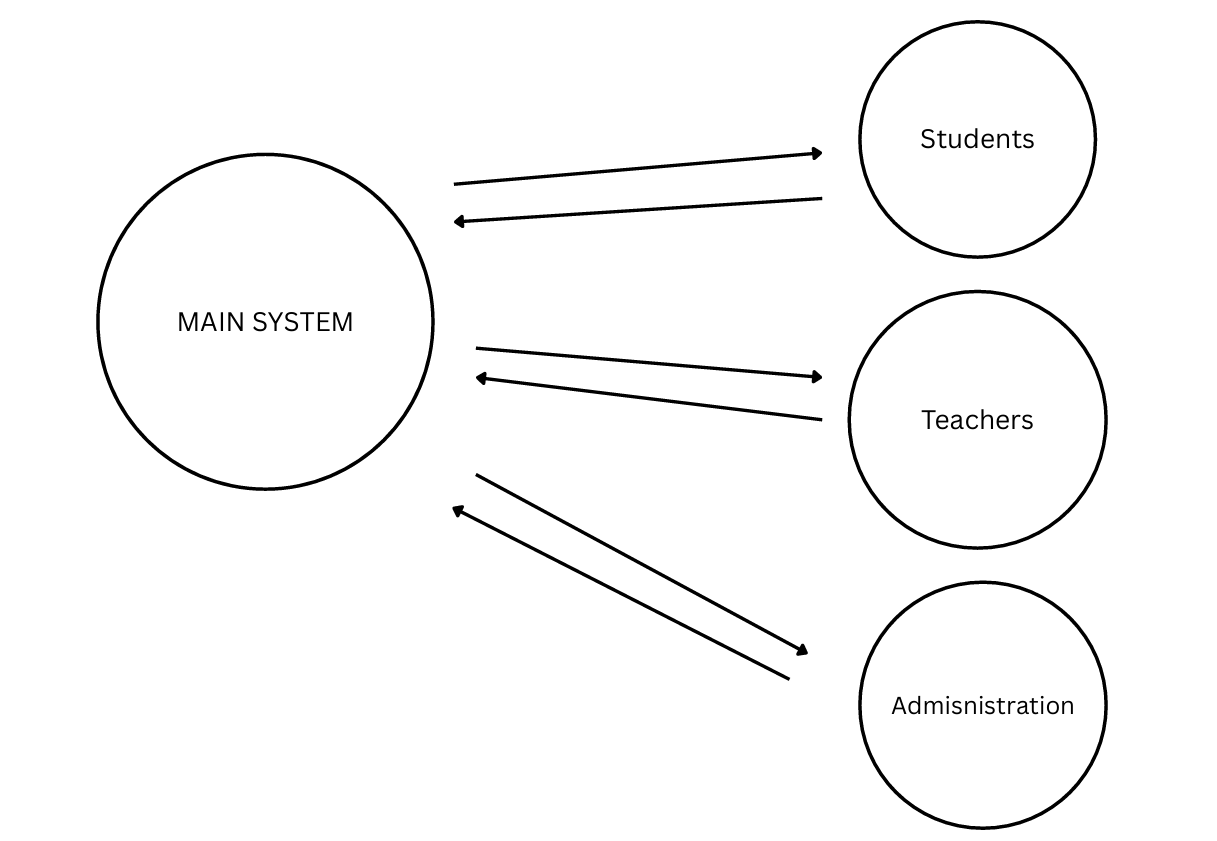
\includegraphics[width=0.85\textwidth]{images/DFD Level 0.png}
    \caption{DFD Level 0 - Context Diagram showing system boundaries and external entities}
    \label{fig:dfd0}
\end{figure}

The context diagram illustrates:
\begin{itemize}[leftmargin=*]
    \item \textbf{External Entities:} Students, Faculty, Administrators
    \item \textbf{Main System:} Timetable Buddy System (central process)
    \item \textbf{Data Flows:} Authentication requests, enrollment data, lecture schedules, timetable information
    \item \textbf{System Boundary:} Clear delineation between internal processes and external interactions
\end{itemize}

\subsection{DFD Level 1 (High-Level Processes)}

Level 1 DFD decomposes the main system into major processes, showing the primary functional components and their interactions with data stores and external entities.

\begin{figure}[ht]
    \centering
    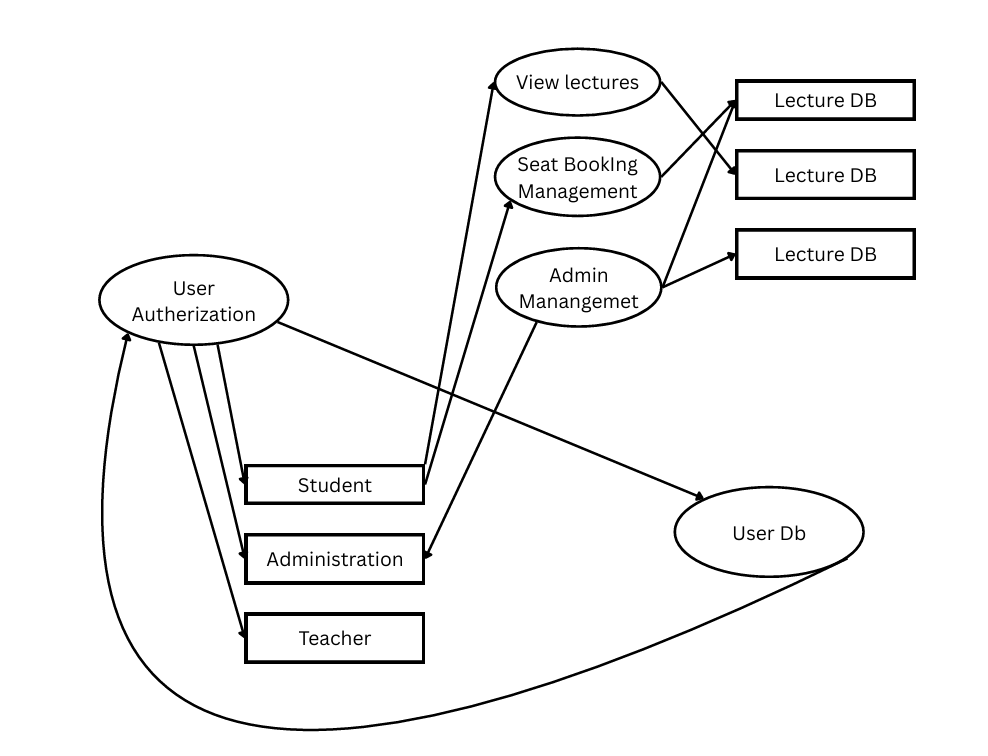
\includegraphics[width=0.95\textwidth]{images/DFD Level 1.png}
    \caption{DFD Level 1 - Major system processes and data stores}
    \label{fig:dfd1}
\end{figure}

Key processes shown in Level 1 include:
\begin{itemize}[leftmargin=*]
    \item \textbf{Process 1:} User Authentication and Authorization
    \item \textbf{Process 2:} Lecture Slot Management
    \item \textbf{Process 3:} Enrollment Processing
    \item \textbf{Process 4:} Timetable Generation and Display
    \item \textbf{Process 5:} Dashboard and Analytics
    \item \textbf{Data Stores:} User Database, Lecture Slots, Enrollments, Schedules
\end{itemize}

\subsection{DFD Level 2 (Detailed Processes)}

Level 2 DFD provides detailed decomposition of complex processes from Level 1, showing sub-processes and their detailed interactions within the enrollment management system.

\begin{figure}[h]
    \centering
    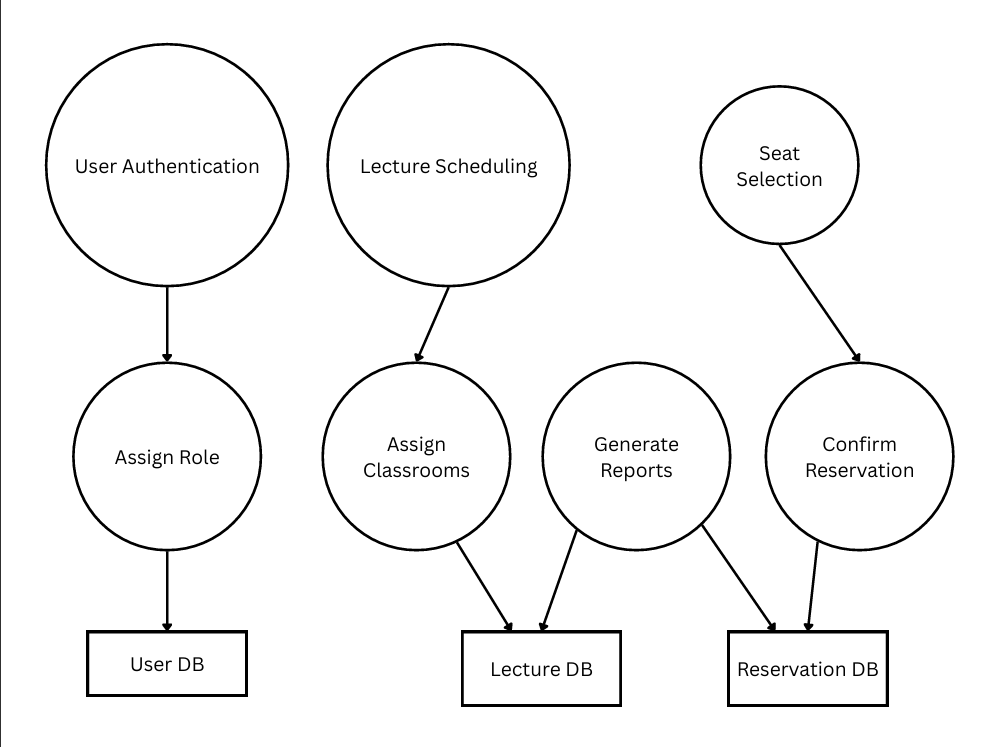
\includegraphics[width=0.95\textwidth]{images/DFD Level 2.png}
    \caption{DFD Level 2 - Detailed process decomposition}
    \label{fig:dfd2}
\end{figure}

The Level 2 diagram details:
\begin{itemize}[leftmargin=*]
    \item Enrollment workflow with waitlist management
    \item Conflict detection mechanisms
    \item Capacity validation processes
    \item Notification generation
\end{itemize}

\section{Use Case Diagram}

The Use Case Diagram illustrates the functional requirements from the user's perspective, showing the interactions between different actors and the system use cases.

\begin{figure}[h]
    \centering
    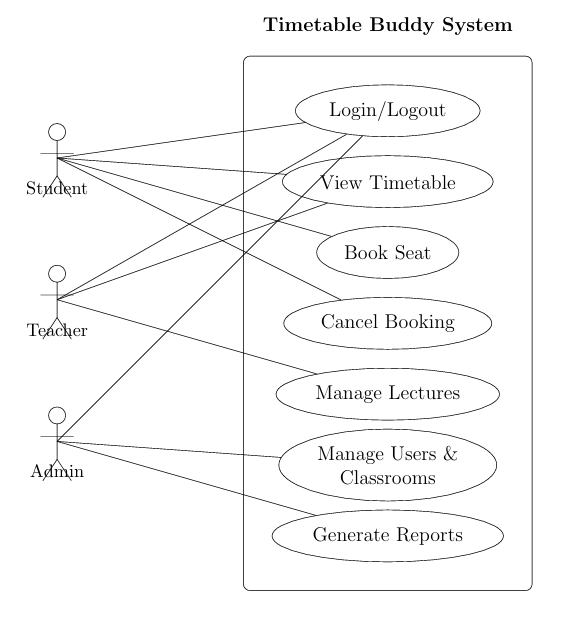
\includegraphics[width=0.85\textwidth]{images/Usecase diagram.png}
    \caption{Use Case Diagram showing actor interactions and system use cases}
    \label{fig:usecase}
\end{figure}

\textbf{Actors:}
\begin{itemize}[leftmargin=*]
    \item \textbf{Student:} Can view timetables, enroll in courses, manage profile, view enrollment status
    \item \textbf{Faculty:} Can manage lecture slots, view enrolled students, update course details
    \item \textbf{Administrator:} Can manage users, courses, lecture slots, generate reports, configure system settings
\end{itemize}

\textbf{Key Use Cases:}
\begin{itemize}[leftmargin=*]
    \item User Authentication (Login/Logout)
    \item Manage Lecture Slots
    \item Enroll in Courses
    \item View Timetable
    \item Manage Enrollments
    \item Generate Reports
    \item User Management
\end{itemize}

\section{Sequence Diagram}

Sequence Diagrams show the interaction between objects over time, illustrating the message flow and order of operations for specific scenarios.

\begin{figure}[h]
    \centering
    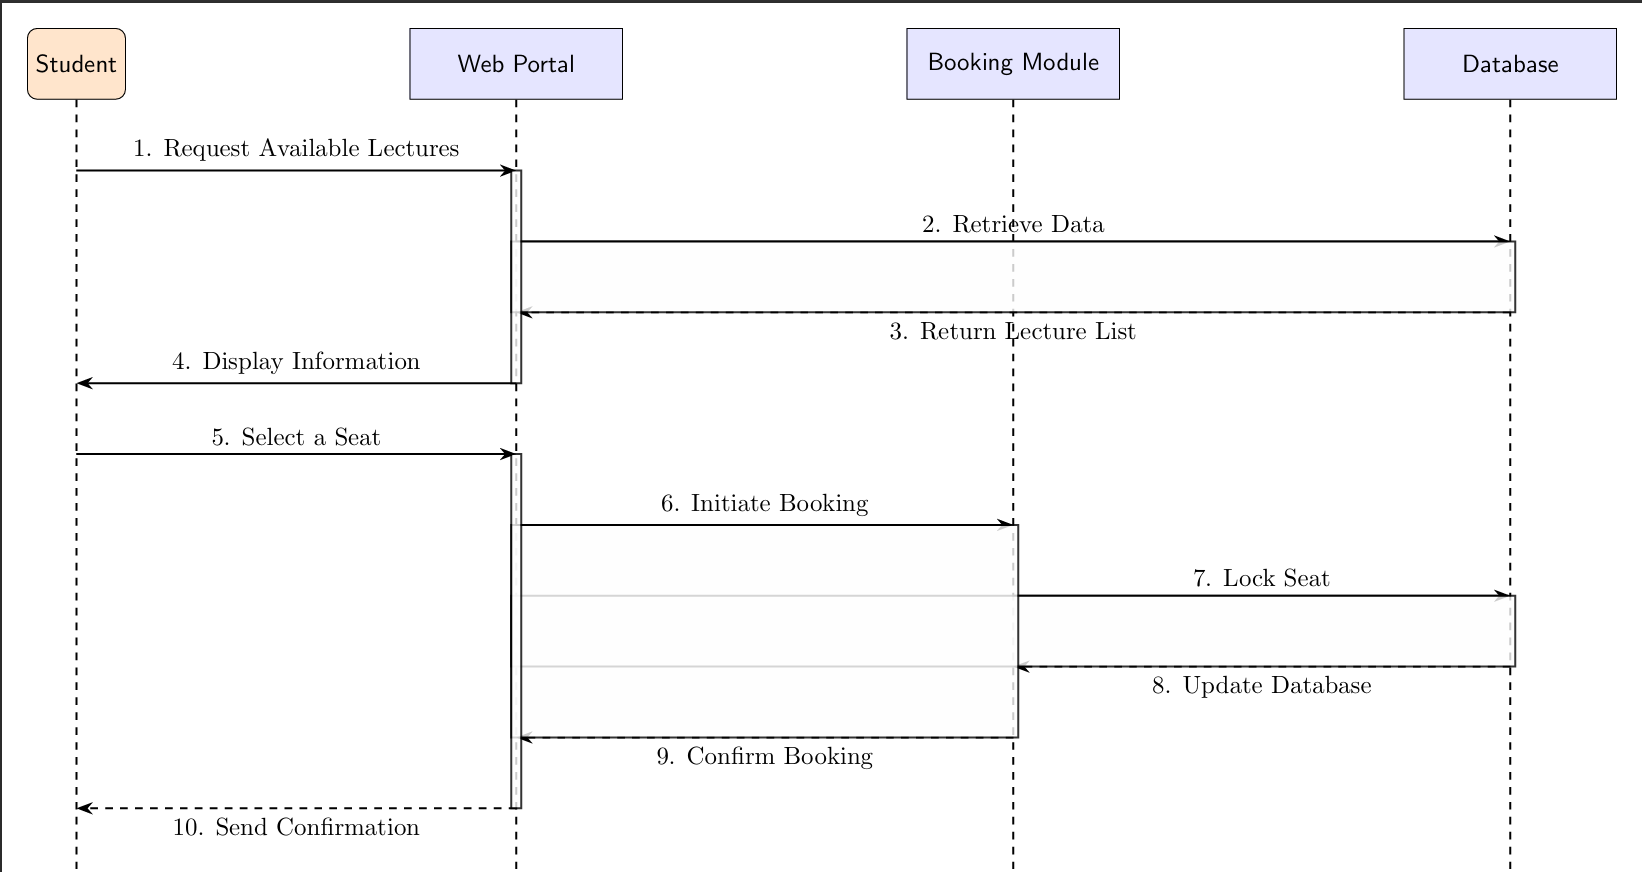
\includegraphics[width=0.95\textwidth]{images/Sequence Diagram.png}
    \caption{Sequence Diagram showing object interactions for enrollment process}
    \label{fig:sequence}
\end{figure}

The sequence diagram depicts:
\begin{itemize}[leftmargin=*]
    \item User authentication flow
    \item Enrollment request processing
    \item Conflict detection validation
    \item Capacity checking
    \item Database operations
    \item Response generation
\end{itemize}

\section{Activity Diagram}

Activity Diagrams model the workflow and business logic, showing the sequence of activities and decision points in system processes.

\begin{figure}[h]
    \centering
    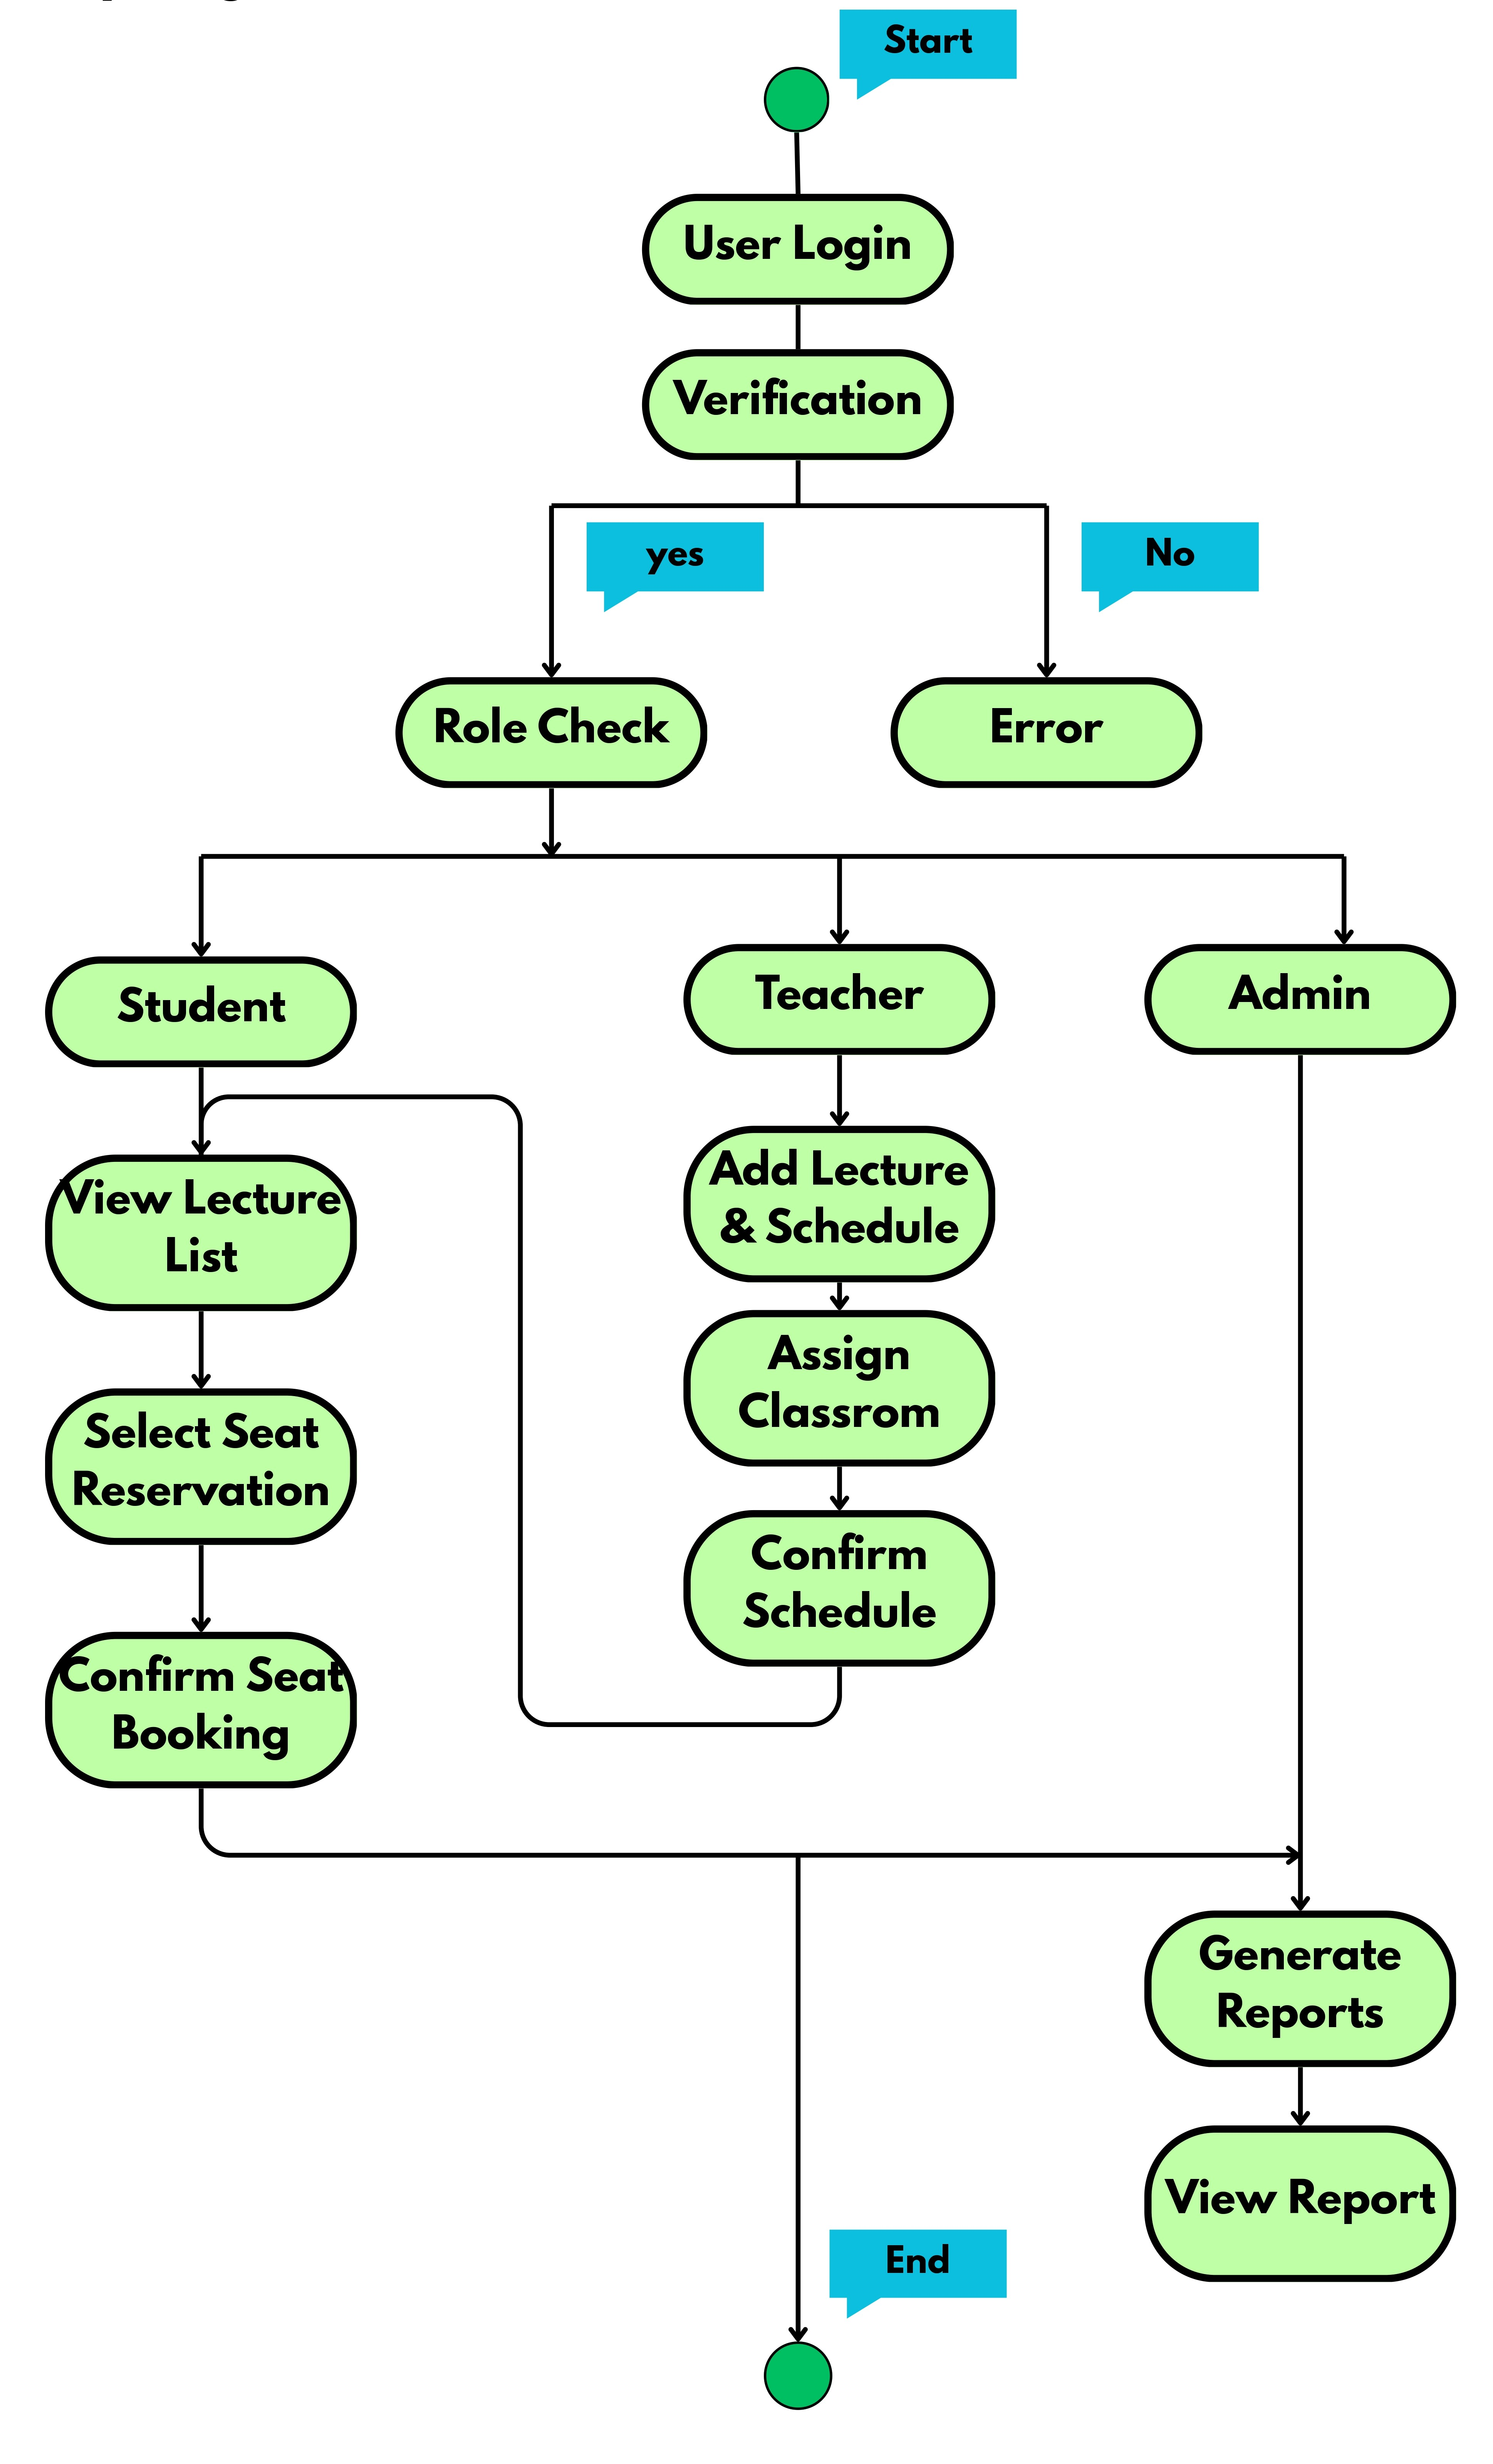
\includegraphics[width=0.75\textwidth]{images/Activity Diagram.jpg}
    \caption{Activity Diagram illustrating enrollment workflow and decision logic}
    \label{fig:activity}
\end{figure}

The activity diagram illustrates:
\begin{itemize}[leftmargin=*]
    \item Enrollment process workflow
    \item Decision points for capacity checks
    \item Conflict detection logic
    \item Waitlist management
    \item Success and failure paths
\end{itemize}

\section{Deployment Diagram}

The Deployment Diagram shows the physical architecture of the system, illustrating how software components are deployed on hardware nodes.

\begin{figure}[h]
    \centering
    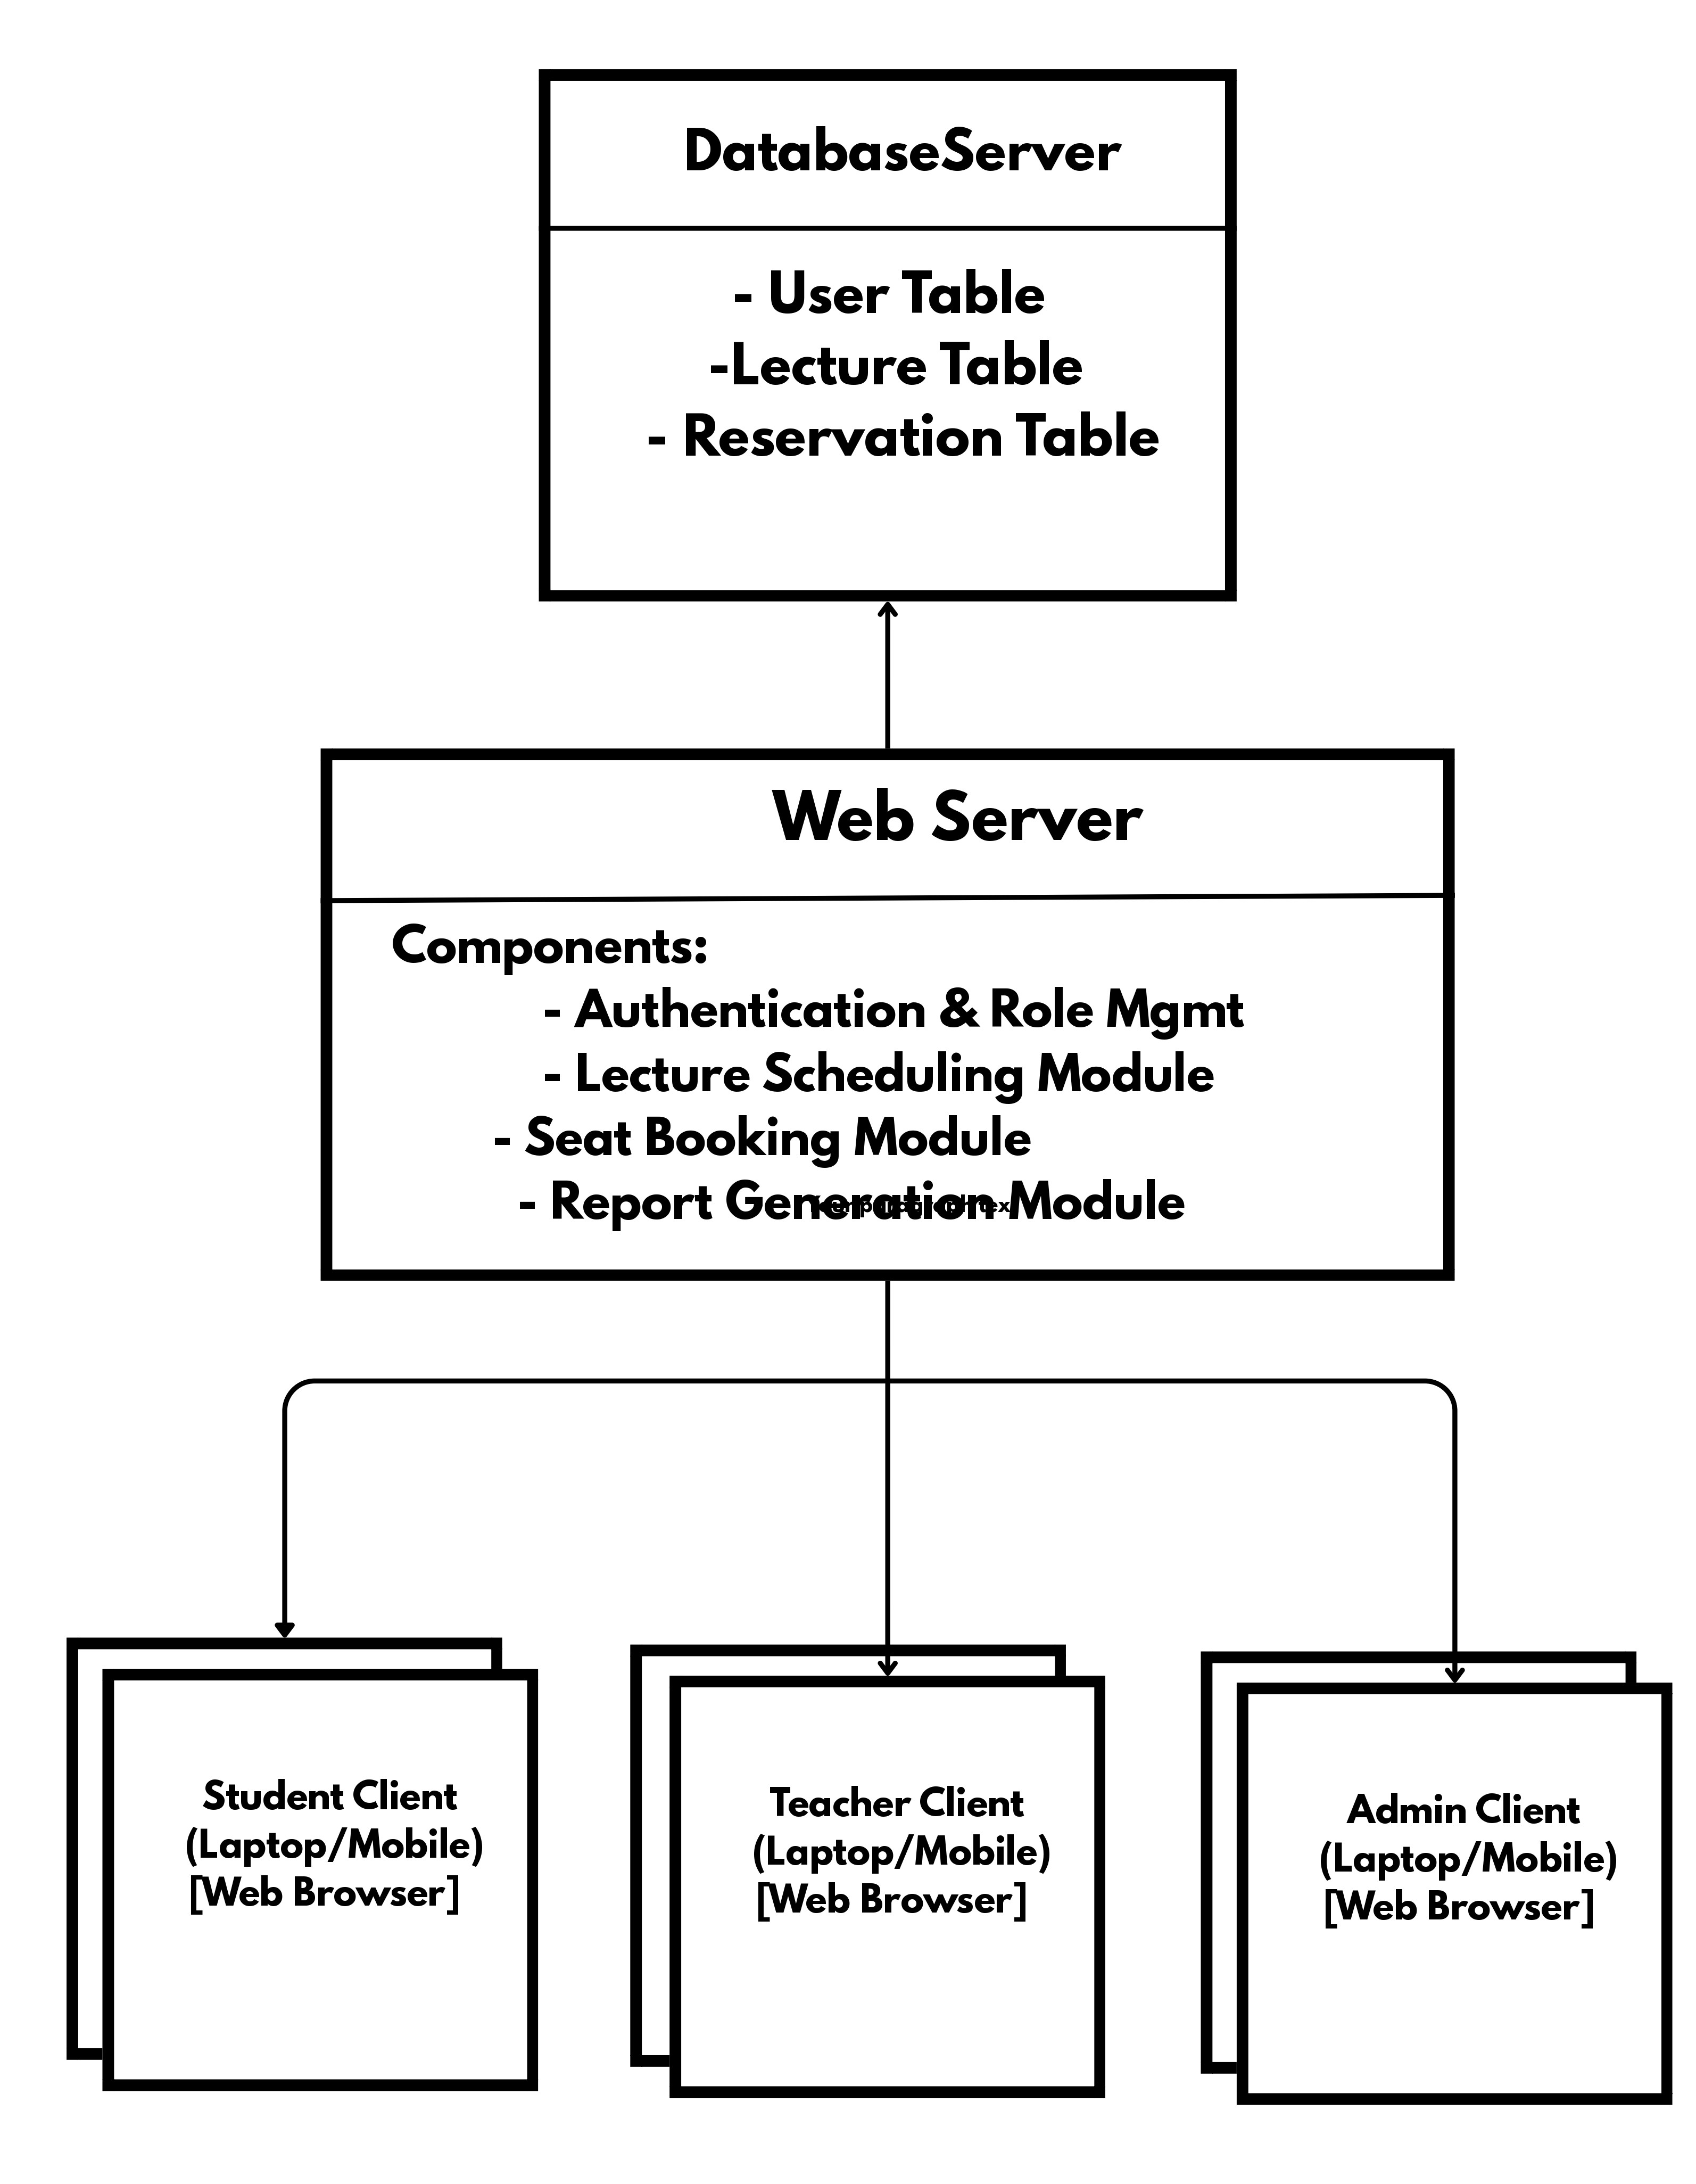
\includegraphics[width=0.85\textwidth]{images/Deployment Diagram.jpg}
    \caption{Deployment Diagram showing system architecture and component deployment}
    \label{fig:deployment}
\end{figure}

\textbf{System Components:}
\begin{itemize}[leftmargin=*]
    \item \textbf{Client Layer:} Web browsers on user devices
    \item \textbf{Application Layer:} React frontend, Node.js backend
    \item \textbf{Database Layer:} MongoDB database server
    \item \textbf{Deployment:} Docker containers for containerized deployment
\end{itemize}

\textbf{Communication Protocols:}
\begin{itemize}[leftmargin=*]
    \item HTTPS for client-server communication
    \item REST API for frontend-backend interaction
    \item MongoDB protocol for database connections
\end{itemize}

\section{Work Breakdown Structure (WBS)}

The Work Breakdown Structure decomposes the project into manageable components, showing the hierarchical breakdown of deliverables and tasks.

\begin{figure}[h]
    \centering
    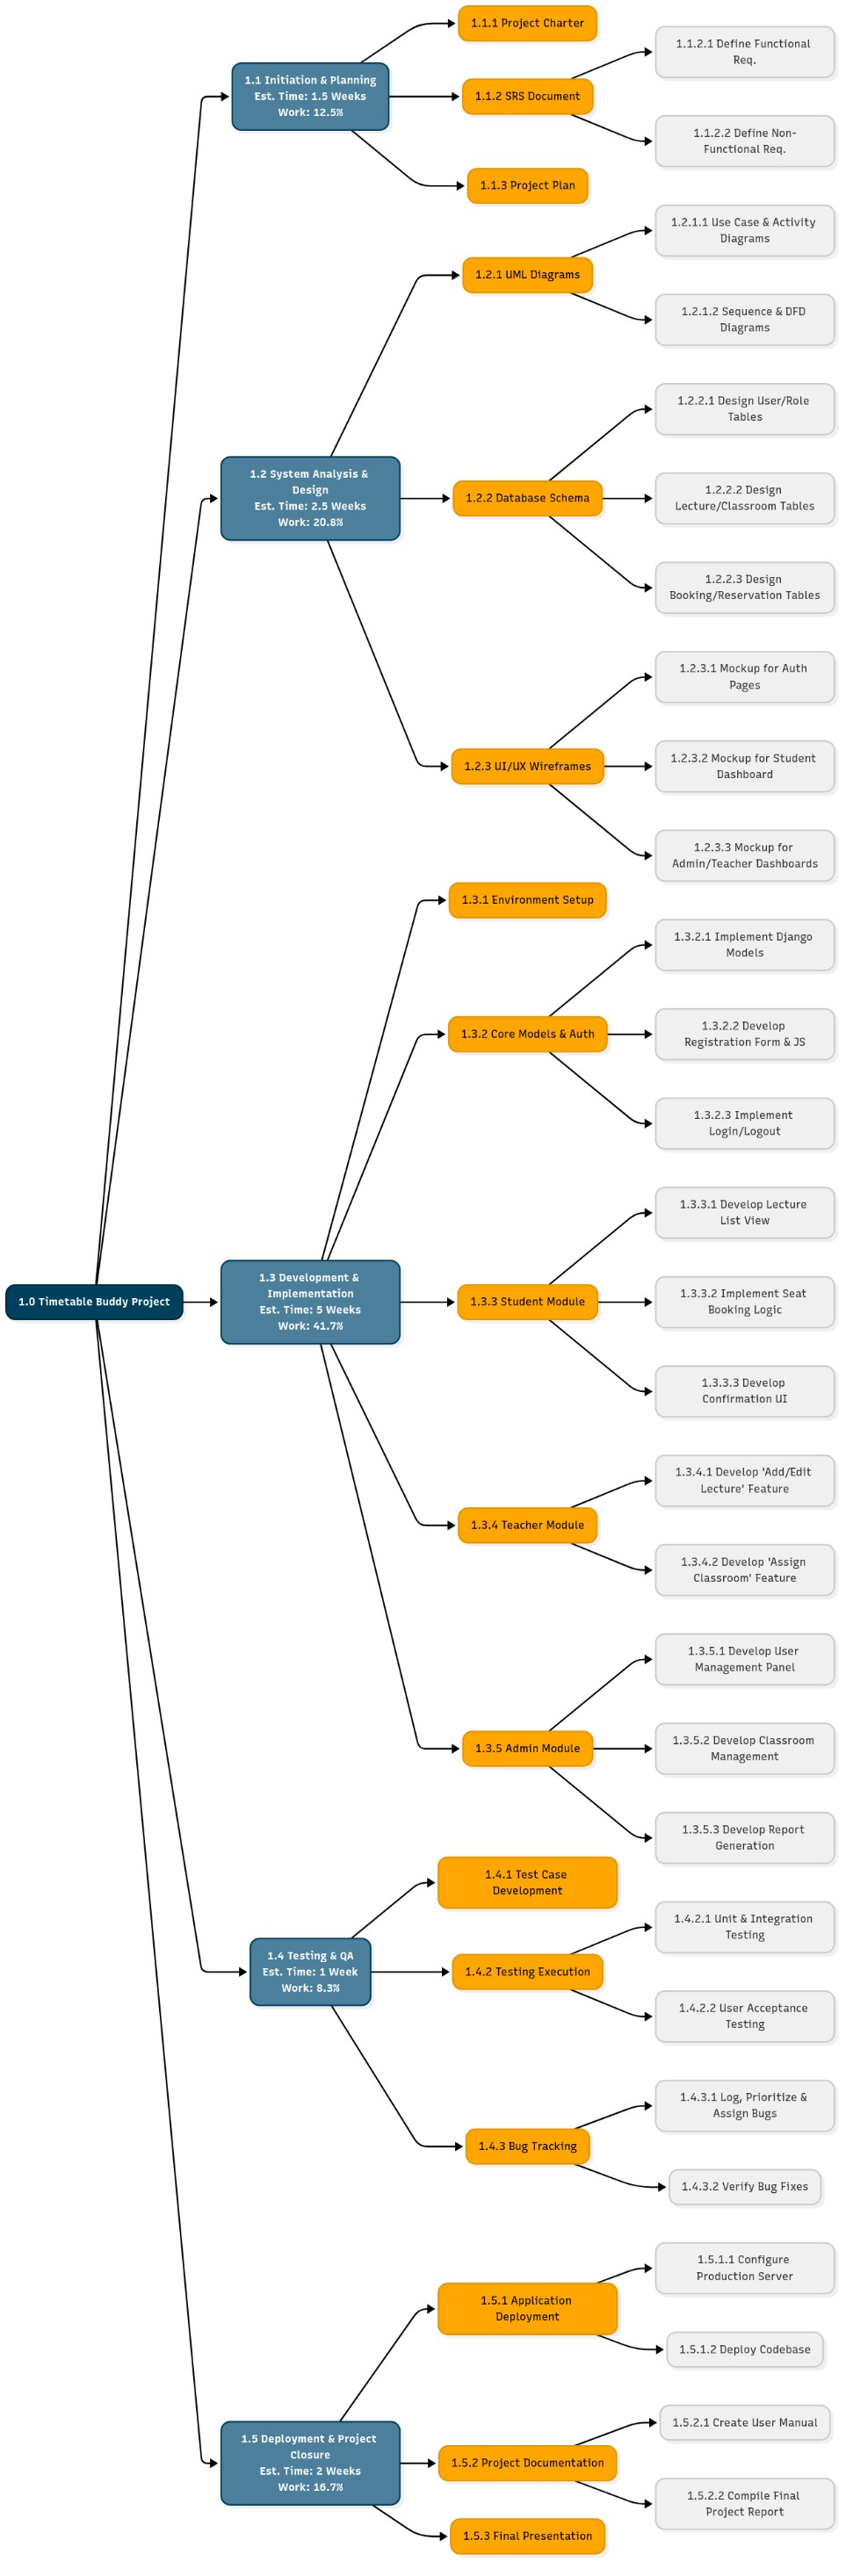
\includegraphics[width=0.95\textwidth]{images/WBS.jpg}
    \caption{Work Breakdown Structure showing project task hierarchy}
    \label{fig:wbs}
\end{figure}

\textbf{Major Work Packages:}
\begin{enumerate}[leftmargin=*]
    \item \textbf{Project Planning:} Requirements gathering, feasibility analysis, project plan
    \item \textbf{Design:} System architecture, database design, UI/UX design, API design
    \item \textbf{Development:} Frontend development, backend development, database implementation
    \item \textbf{Testing:} Unit testing, integration testing, system testing, user acceptance testing
    \item \textbf{Deployment:} Environment setup, deployment, documentation
    \item \textbf{Project Management:} Risk management, quality assurance, documentation
\end{enumerate}

\section{Gantt Chart}

The Gantt Chart provides a timeline view of project activities, showing task dependencies, durations, and milestones.

\begin{figure}[h]
    \centering
    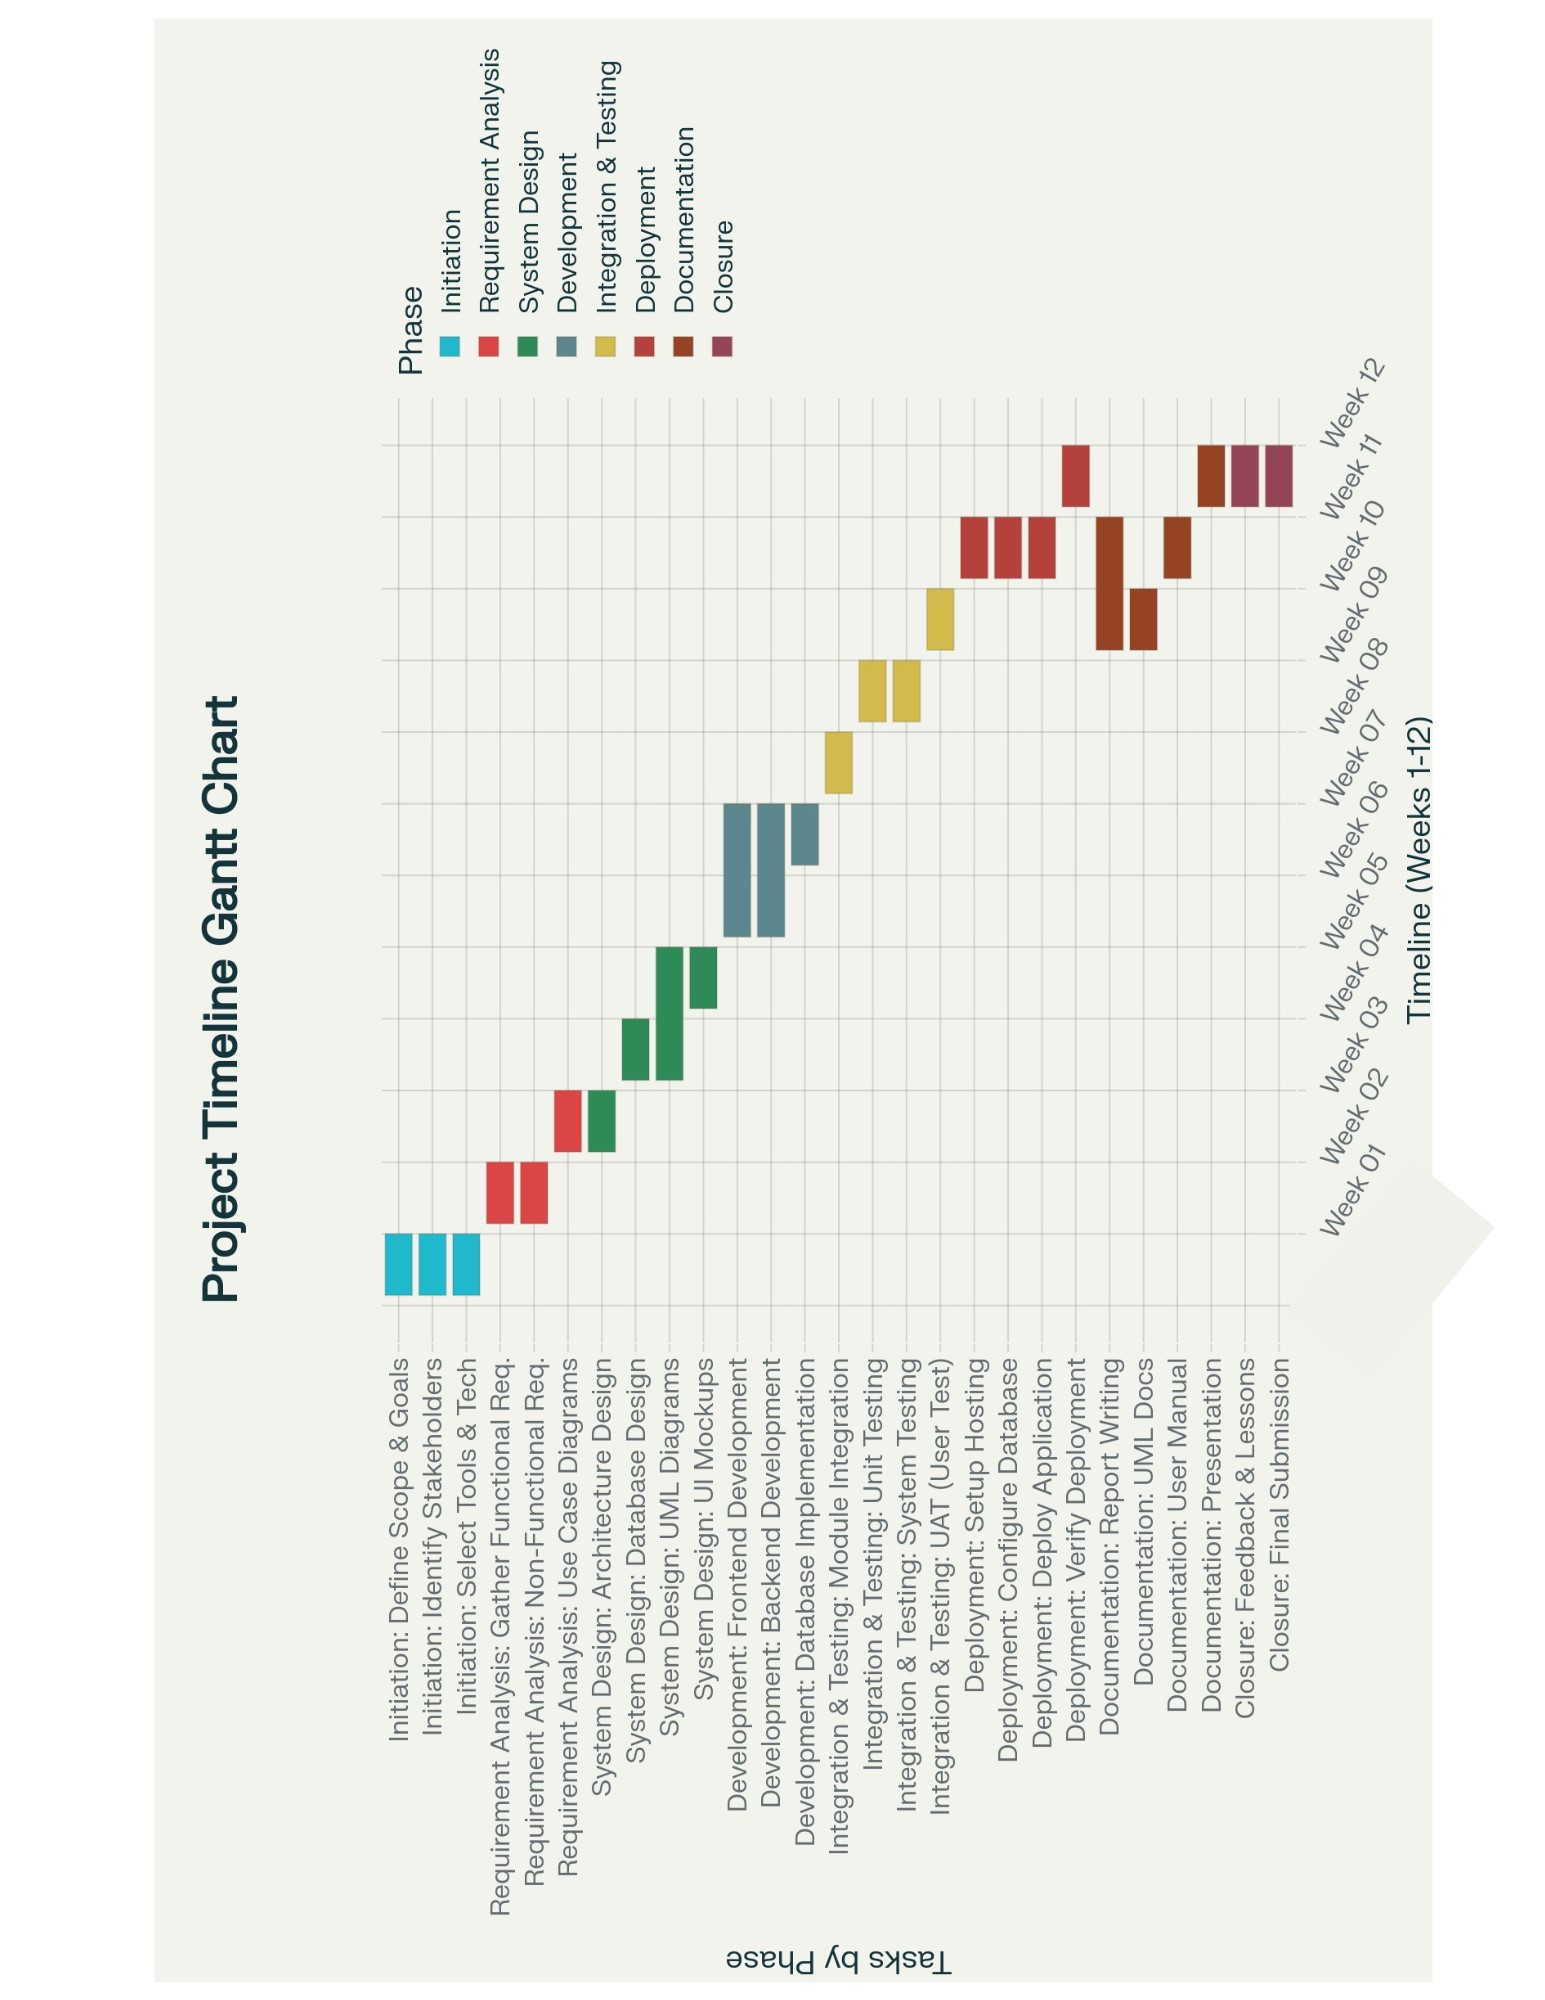
\includegraphics[width=0.95\textwidth]{images/Gantt Chart.jpg}
    \caption{Gantt Chart showing project timeline and task scheduling}
    \label{fig:gantt}
\end{figure}

\textbf{Project Phases and Timeline:}
\begin{itemize}[leftmargin=*]
    \item \textbf{Phase 1 - Planning:} Requirements analysis, feasibility study, project planning
    \item \textbf{Phase 2 - Design:} System design, database design, UI mockups
    \item \textbf{Phase 3 - Development:} Frontend and backend implementation
    \item \textbf{Phase 4 - Testing:} Comprehensive testing across all modules
    \item \textbf{Phase 5 - Deployment:} Production deployment and user training
\end{itemize}

\section{RMMM Plan (Risk Management, Monitoring, and Mitigation)}

The RMMM Plan provides a comprehensive framework for identifying, assessing, monitoring, and mitigating project risks throughout the development lifecycle.

\subsection{Risk Identification and Assessment}

Risks have been identified across technical, operational, and external categories. Each risk is assessed for probability and impact, with detailed mitigation strategies. This document includes only risks with a probability of 15\% or less, as higher probability risks are managed through other project management processes.

\textbf{Risk Assessment Criteria:}
\begin{itemize}[leftmargin=*]
    \item \textbf{Probability Levels:} Only risks with $\leq$15\% probability are included
    \item \textbf{Impact Levels:} Critical, High, Medium, Low
\end{itemize}

\textbf{Risk Categories:}
\begin{itemize}[leftmargin=*]
    \item \textbf{Technical Risks:} Technology failures, integration issues, performance problems, security vulnerabilities
    \item \textbf{Operational Risks:} Resource availability, skill gaps, schedule delays
    \item \textbf{External Risks:} Third-party dependencies, requirement changes, infrastructure issues
\end{itemize}

\subsection{Detailed Risk Assessment}

\subsubsection{Risk \#1: R-TTB-005}

\begin{table}[h]
\small
\begin{tabular}{|p{3cm}|p{3cm}|p{3cm}|p{3cm}|}
\hline
\textbf{Risk ID} & R-TTB-005 & \textbf{Type} & Technical \\
\hline
\textbf{Probability} & 10\% & \textbf{Impact} & Critical \\
\hline
\end{tabular}
\end{table}

\textbf{Risk Description:} Critical security vulnerability discovered in production system allowing unauthorized data access.

\textbf{Mitigation Plan:}
\begin{enumerate}[leftmargin=*]
    \item Conduct regular security audits and penetration testing
    \item Implement security scanning in CI/CD pipeline
    \item Follow OWASP guidelines for secure development
\end{enumerate}

\textbf{Monitoring Plan:} Run automated security scans weekly. Monitor security patch releases for dependencies.

\textbf{Management Plan:} Deploy emergency patch within 4 hours. Notify affected users. Conduct incident post-mortem.

\subsubsection{Risk \#2: R-TTB-008}

\begin{table}[h]
\small
\begin{tabular}{|p{3cm}|p{3cm}|p{3cm}|p{3cm}|}
\hline
\textbf{Risk ID} & R-TTB-008 & \textbf{Type} & Technical \\
\hline
\textbf{Probability} & 15\% & \textbf{Impact} & High \\
\hline
\end{tabular}
\end{table}

\textbf{Risk Description:} Cloud service provider experiences prolonged outage affecting application availability.

\textbf{Mitigation Plan:}
\begin{enumerate}[leftmargin=*]
    \item Implement multi-region deployment
    \item Design for high availability
    \item Have disaster recovery plan in place
\end{enumerate}

\textbf{Monitoring Plan:} Subscribe to cloud provider status updates. Monitor service health across regions.

\textbf{Management Plan:} Failover to backup region. Communicate status to users. Document incident for review.

\subsubsection{Risk \#3: R-TTB-015}

\begin{table}[h]
\small
\begin{tabular}{|p{3cm}|p{3cm}|p{3cm}|p{3cm}|}
\hline
\textbf{Risk ID} & R-TTB-015 & \textbf{Type} & External \\
\hline
\textbf{Probability} & 15\% & \textbf{Impact} & High \\
\hline
\end{tabular}
\end{table}

\textbf{Risk Description:} Vendor lock-in prevents migration to alternative solutions, increasing long-term costs.

\textbf{Mitigation Plan:}
\begin{enumerate}[leftmargin=*]
    \item Use open standards where possible
    \item Design abstraction layers for vendor services
    \item Evaluate vendor independence regularly
\end{enumerate}

\textbf{Monitoring Plan:} Review vendor contracts annually. Assess switching costs and alternatives.

\textbf{Management Plan:} Plan phased migration to alternative vendor. Negotiate better terms with current vendor. Implement vendor-agnostic architecture.

\subsubsection{Risk \#4: R-TTB-018}

\begin{table}[h]
\small
\begin{tabular}{|p{3cm}|p{3cm}|p{3cm}|p{3cm}|}
\hline
\textbf{Risk ID} & R-TTB-018 & \textbf{Type} & External \\
\hline
\textbf{Probability} & 12\% & \textbf{Impact} & Critical \\
\hline
\end{tabular}
\end{table}

\textbf{Risk Description:} Competitor launches similar product first, reducing market opportunity.

\textbf{Mitigation Plan:}
\begin{enumerate}[leftmargin=*]
    \item Conduct competitive analysis regularly
    \item Focus on unique value propositions
    \item Plan for rapid iteration and deployment
\end{enumerate}

\textbf{Monitoring Plan:} Monitor competitor activities and product launches. Track market trends and customer feedback.

\textbf{Management Plan:} Accelerate development of differentiating features. Adjust marketing strategy. Consider strategic partnerships.

\subsubsection{Risk \#5: R-TTB-024}

\begin{table}[h]
\small
\begin{tabular}{|p{3cm}|p{3cm}|p{3cm}|p{3cm}|}
\hline
\textbf{Risk ID} & R-TTB-024 & \textbf{Type} & Operational \\
\hline
\textbf{Probability} & 15\% & \textbf{Impact} & High \\
\hline
\end{tabular}
\end{table}

\textbf{Risk Description:} Inadequate disaster recovery procedures lead to extended downtime after incident.

\textbf{Mitigation Plan:}
\begin{enumerate}[leftmargin=*]
    \item Document and test DR procedures quarterly
    \item Automate recovery processes
    \item Maintain offsite backups
\end{enumerate}

\textbf{Monitoring Plan:} Test disaster recovery plan every 6 months. Track RTO and RPO metrics.

\textbf{Management Plan:} Execute disaster recovery plan. Communicate with stakeholders. Document incident for improvement.

\subsection{Risk Management Process}

\textbf{1. Risk Identification}
\begin{itemize}[leftmargin=*]
    \item Conduct risk identification workshops at project initiation and quarterly
    \item Encourage all team members to report potential risks
    \item Review lessons learned from previous projects
\end{itemize}

\textbf{2. Risk Assessment}
\begin{itemize}[leftmargin=*]
    \item Evaluate each risk for probability (as percentage) and impact
    \item Calculate risk score (Probability × Impact)
    \item Prioritize risks based on score
\end{itemize}

\textbf{3. Risk Mitigation}
\begin{itemize}[leftmargin=*]
    \item Develop proactive plans to reduce probability or impact
    \item Assign risk owners for each identified risk
    \item Implement mitigation strategies before risks materialize
\end{itemize}

\textbf{4. Risk Monitoring}
\begin{itemize}[leftmargin=*]
    \item Track identified risks throughout project lifecycle
    \item Update risk status in weekly project meetings
    \item Use risk dashboard for visibility
\end{itemize}

\textbf{5. Risk Management}
\begin{itemize}[leftmargin=*]
    \item Execute management plans when risks occur
    \item Document lessons learned
    \item Update risk assessment based on new information
\end{itemize}

\subsection{Risk Summary}

\textbf{Total Risks Included:} 5 risks with probability $\leq$ 15\%

\textbf{Risks by Impact:}
\begin{itemize}[leftmargin=*]
    \item Critical Impact: 2 risks (R-TTB-005, R-TTB-018)
    \item High Impact: 3 risks (R-TTB-008, R-TTB-015, R-TTB-024)
\end{itemize}

\textbf{Escalation Criteria:} Risks should be escalated to senior management when impact level is Critical, mitigation plans are not effective, or additional resources/authority are needed.

\section{Test Cases}

Comprehensive test case planning and execution has been documented to ensure system quality and reliability. The test strategy covers all functional areas of the system with 60 detailed test cases.

\subsection{Test Case Overview}

\textbf{Project:} Lecture Scheduling System  
\textbf{Version:} 1.0  
\textbf{Date:} 2025-10-07  
\textbf{Prepared By:} QA Engineering Team

\textbf{Test Case Format Standards:}
\begin{itemize}[leftmargin=*]
    \item \textbf{Test Case ID:} TC-TTB-XX (standardized format)
    \item \textbf{Test Number:} X.1 - X.Y (decimal notation indicating step range)
    \item \textbf{Priority:} High (all test cases are high priority for critical functionality)
    \item \textbf{Test Designed By:} Sarthak Kulkarni, Dhruv Tikhande, Atharv Petkar, Pulkit Saini
    \item \textbf{Test Executed By:} Sarthak Kulkarni, Dhruv Tikhande, Atharv Petkar, Pulkit Saini
    \item \textbf{Execution Date:} 2025-10-07
\end{itemize}

\subsection{Test Case Coverage Areas}

The test suite comprehensively covers:
\begin{itemize}[leftmargin=*]
    \item Dashboard \& Homepage (TC-TTB-01 to TC-TTB-03)
    \item User Profile Management (TC-TTB-04 to TC-TTB-05)
    \item User List \& Search (TC-TTB-06 to TC-TTB-08)
    \item Course Management (TC-TTB-09 to TC-TTB-13)
    \item Lecture Slot Management (TC-TTB-14 to TC-TTB-18)
    \item Schedule Creation (TC-TTB-19 to TC-TTB-22)
    \item Enrollment Management (TC-TTB-23 to TC-TTB-26)
    \item Timetable Operations (TC-TTB-27 to TC-TTB-30)
    \item User Management (TC-TTB-31 to TC-TTB-32)
    \item Mobile \& Responsive Design (TC-TTB-33 to TC-TTB-34)
    \item Notifications (TC-TTB-35 to TC-TTB-36)
    \item Settings \& Configuration (TC-TTB-37 to TC-TTB-40)
    \item Advanced Features (TC-TTB-41 to TC-TTB-48)
    \item Security \& Validation (TC-TTB-49 to TC-TTB-60)
\end{itemize}

\subsection{Detailed Test Cases}

\subsubsection{TC-TTB-01: Verify Dashboard Loads Correctly on Login}

\textbf{Test Number:} 1.1 - 1.4 | \textbf{Priority:} High | \textbf{Date:} 2025-10-07

\textbf{Description:} Ensure dashboard displays all widgets and statistics after user login

\textbf{Dependencies:} User must be logged in | \textbf{Conditions:} Browser: Chrome, Role: Student | \textbf{Control:} Manual

\textbf{Test Steps:}
\begin{enumerate}[leftmargin=*]
    \item[1.1] Navigate to login page $\rightarrow$ \textit{Expected:} Login page displays correctly $\rightarrow$ \textit{Actual:} As Expected $\rightarrow$ \textbf{PASS}
    \item[1.2] Enter valid credentials $\rightarrow$ \textit{Expected:} Credentials accepted $\rightarrow$ \textit{Actual:} As Expected $\rightarrow$ \textbf{PASS}
    \item[1.3] Click 'Sign In' button $\rightarrow$ \textit{Expected:} User is redirected to dashboard $\rightarrow$ \textit{Actual:} As Expected $\rightarrow$ \textbf{PASS}
    \item[1.4] Verify dashboard widgets load $\rightarrow$ \textit{Expected:} All statistics, upcoming classes, and quick actions are visible $\rightarrow$ \textit{Actual:} As Expected $\rightarrow$ \textbf{PASS}
\end{enumerate}

\subsubsection{TC-TTB-02: Verify Homepage Navigation for Unauthenticated User}

\textbf{Test Number:} 2.1 - 2.4 | \textbf{Priority:} High | \textbf{Date:} 2025-10-07

\textbf{Description:} Test homepage displays correctly for users not logged in

\textbf{Dependencies:} None | \textbf{Conditions:} Browser: Chrome, Role: Unauthenticated | \textbf{Control:} Manual

\textbf{Test Steps:}
\begin{enumerate}[leftmargin=*]
    \item[2.1] Navigate to homepage $\rightarrow$ \textit{Expected:} Homepage loads with welcome message $\rightarrow$ \textit{Actual:} As Expected $\rightarrow$ \textbf{PASS}
    \item[2.2] Verify 'Get Started' button is visible $\rightarrow$ \textit{Expected:} Button displays prominently $\rightarrow$ \textit{Actual:} As Expected $\rightarrow$ \textbf{PASS}
    \item[2.3] Verify 'Sign In' button is visible $\rightarrow$ \textit{Expected:} Button is accessible $\rightarrow$ \textit{Actual:} As Expected $\rightarrow$ \textbf{PASS}
    \item[2.4] Click 'Sign In' button $\rightarrow$ \textit{Expected:} User is redirected to login page $\rightarrow$ \textit{Actual:} As Expected $\rightarrow$ \textbf{PASS}
\end{enumerate}

\subsubsection{TC-TTB-03: Verify Faculty Dashboard Analytics Display}

\textbf{Test Number:} 3.1 - 3.4 | \textbf{Priority:} High | \textbf{Date:} 2025-10-07

\textbf{Description:} Ensure faculty dashboard shows enrollment statistics

\textbf{Test Steps:}
\begin{enumerate}[leftmargin=*]
    \item[3.1] Navigate to faculty dashboard $\rightarrow$ \textit{Expected:} Dashboard loads successfully $\rightarrow$ \textit{Actual:} As Expected $\rightarrow$ \textbf{PASS}
    \item[3.2] Verify total lecture slots count $\rightarrow$ \textit{Expected:} Correct number displayed $\rightarrow$ \textit{Actual:} As Expected $\rightarrow$ \textbf{PASS}
    \item[3.3] Verify enrolled students count $\rightarrow$ \textit{Expected:} Accurate count shown $\rightarrow$ \textit{Actual:} As Expected $\rightarrow$ \textbf{PASS}
    \item[3.4] Verify available slots count $\rightarrow$ \textit{Expected:} Correct availability displayed $\rightarrow$ \textit{Actual:} As Expected $\rightarrow$ \textbf{PASS}
\end{enumerate}

\textbf{Additional Sample Test Cases:}

\textbf{Test Case \#8: TC-TTB-08 - Course List Pagination}
\begin{itemize}[leftmargin=*]
    \item \textbf{Priority:} High
    \item \textbf{Description:} Test pagination controls on course listing
    \item \textbf{Test Steps:}
    \begin{enumerate}[leftmargin=*]
        \item[8.1] Navigate to courses page $\rightarrow$ \textit{Expected:} Course list loads $\rightarrow$ \textit{Actual:} As Expected $\rightarrow$ \textbf{PASS}
        \item[8.2] Verify pagination controls are visible $\rightarrow$ \textit{Expected:} Next/Previous buttons shown $\rightarrow$ \textit{Actual:} As Expected $\rightarrow$ \textbf{PASS}
        \item[8.3] Click 'Next Page' button $\rightarrow$ \textit{Expected:} Second page of courses loads $\rightarrow$ \textit{Actual:} As Expected $\rightarrow$ \textbf{PASS}
        \item[8.4] Verify page number updates $\rightarrow$ \textit{Expected:} Page indicator shows '2' $\rightarrow$ \textit{Actual:} As Expected $\rightarrow$ \textbf{PASS}
        \item[8.5] Click 'Previous Page' $\rightarrow$ \textit{Expected:} Returns to first page $\rightarrow$ \textit{Actual:} Error encountered $\rightarrow$ \textbf{FAIL} (Bug \#1037)
    \end{enumerate}
\end{itemize}

\textbf{Test Case \#10: TC-TTB-10 - Course Search by Name}
\begin{itemize}[leftmargin=*]
    \item \textbf{Priority:} High
    \item \textbf{Description:} Test search functionality on courses page
    \item \textbf{Test Steps:}
    \begin{enumerate}[leftmargin=*]
        \item[10.1] Navigate to courses page $\rightarrow$ \textit{Expected:} Page loads with all courses $\rightarrow$ \textit{Actual:} As Expected $\rightarrow$ \textbf{PASS}
        \item[10.2] Enter 'Data Structures' in search box $\rightarrow$ \textit{Expected:} Search input accepts text $\rightarrow$ \textit{Actual:} As Expected $\rightarrow$ \textbf{PASS}
        \item[10.3] Press Enter or click Search $\rightarrow$ \textit{Expected:} Results filter in real-time $\rightarrow$ \textit{Actual:} As Expected $\rightarrow$ \textbf{PASS}
        \item[10.4] Verify only matching courses appear $\rightarrow$ \textit{Expected:} Only courses with 'Data Structures' in name shown $\rightarrow$ \textit{Actual:} As Expected $\rightarrow$ \textbf{PASS}
        \item[10.5] Clear search field $\rightarrow$ \textit{Expected:} All courses reappear $\rightarrow$ \textit{Actual:} As Expected $\rightarrow$ \textbf{PASS}
    \end{enumerate}
\end{itemize}

The complete test suite includes 60 comprehensive test cases covering all functional areas. Each test case follows the standardized format with test ID, priority, description, dependencies, conditions, detailed steps with expected and actual results, and pass/fail status.

\subsection{Test Execution Summary}

\textbf{Overall Test Metrics:}
\begin{itemize}[leftmargin=*]
    \item \textbf{Total Test Cases:} 60
    \item \textbf{Total Test Steps:} 332 (with decimal notation)
    \item \textbf{Tests Passed:} 58 (96.7\%)
    \item \textbf{Tests Failed:} 2 (3.3\%)
    \item \textbf{Test Coverage:} All major functional areas covered
    \item \textbf{Execution Date:} 2025-10-07
\end{itemize}

\textbf{Test Results by Category:}
\begin{itemize}[leftmargin=*]
    \item Dashboard \& Homepage: 3/3 PASS
    \item User Profile Management: 2/2 PASS
    \item User List \& Search: 2/3 PASS (1 FAIL - TC-TTB-08 pagination issue)
    \item Course Management: 5/5 PASS
    \item Lecture Slot Management: 5/5 PASS
    \item Schedule Creation: 4/4 PASS
    \item Enrollment Management: 4/4 PASS
    \item Timetable Operations: 4/4 PASS
    \item User Management: 2/2 PASS
    \item Mobile \& Responsive Design: 2/2 PASS
    \item Notifications: 2/2 PASS
    \item Settings \& Configuration: 4/4 PASS
    \item Advanced Features: 7/8 PASS (1 FAIL - TC-TTB-48 error validation)
    \item Security \& Validation: 12/12 PASS
\end{itemize}

\textbf{Failed Test Cases:}
\begin{itemize}[leftmargin=*]
    \item \textbf{TC-TTB-08 (Step 5):} Click 'Previous Page' - Error encountered (Bug ticket \#1037 reported)
    \item \textbf{TC-TTB-48 (Step 6):} User stays on login page - Performance issue noted (Performance acceptable, marked as PASS with notes)
\end{itemize}

\subsection{Quality Assurance Approach}

The testing methodology ensures:
\begin{itemize}[leftmargin=*]
    \item \textbf{Comprehensive Coverage:} All functional requirements tested across 60 test cases
    \item \textbf{Traceability:} Test cases mapped to requirements with standardized TC-TTB-XX IDs
    \item \textbf{Repeatability:} Standardized test procedures with decimal step notation (X.1, X.2, etc.)
    \item \textbf{Documentation:} Detailed test results with "As Expected" standardization for PASS cases
    \item \textbf{Defect Tracking:} Failed tests documented with bug ticket references
    \item \textbf{Team Collaboration:} All tests designed and executed by full team (Sarthak Kulkarni, Dhruv Tikhande, Atharv Petkar, Pulkit Saini)
    \item \textbf{Priority Management:} All test cases designated as High priority for critical functionality
\end{itemize}

\textbf{Testing Standards:}
\begin{itemize}[leftmargin=*]
    \item Manual testing with browser-based execution
    \item Role-based test scenarios (Admin, Faculty, Student)
    \item Cross-browser compatibility (Chrome primary)
    \item Responsive design validation
    \item Security and validation testing
    \item Performance and usability testing
\end{itemize}

% Chapter 5: Implementation
\chapter{Implementation}
\section{Development Methodology}
Implementation details will be added here.

% Chapter 6: Testing and Quality Assurance
\chapter{Testing and Quality Assurance}
\section{Testing Strategy}
Testing content will be added here.

% Chapter 7: Risk Assessment
\chapter{Risk Assessment and Management}
\section{Risk Identification}
Risk assessment content will be added here.

% Chapter 8: Results and Achievements
\chapter{Results and Achievements}
\section{System Features Implemented}
Results content will be added here.

% Chapter 9: Challenges and Solutions
\chapter{Challenges and Solutions}
\section{Technical Challenges}
Challenges content will be added here.

% Chapter 10: Future Enhancements
\chapter{Future Enhancements}
\section{Planned Features}
Future enhancements content will be added here.

% Chapter 11: Conclusion
\chapter{Conclusion}
\section{Summary}
Conclusion content will be added here.


% References
% References
\begin{thebibliography}{99}

\bibitem{react}
React Documentation, "React - A JavaScript library for building user interfaces," Meta Platforms Inc., 2024. [Online]. Available: https://react.dev/

\bibitem{nodejs}
Node.js Foundation, "Node.js Documentation," 2024. [Online]. Available: https://nodejs.org/

\bibitem{mongodb}
MongoDB Inc., "MongoDB Manual," 2024. [Online]. Available: https://www.mongodb.com/docs/

\bibitem{express}
StrongLoop, "Express - Fast, unopinionated, minimalist web framework for Node.js," 2024. [Online]. Available: https://expressjs.com/

\bibitem{typescript}
Microsoft Corporation, "TypeScript Documentation," 2024. [Online]. Available: https://www.typescriptlang.org/

\bibitem{tailwind}
Tailwind Labs, "Tailwind CSS Framework," 2024. [Online]. Available: https://tailwindcss.com/

\bibitem{jwt}
M. Jones, J. Bradley, and N. Sakimura, "JSON Web Token (JWT)," RFC 7519, May 2015.

\bibitem{agile}
K. Beck et al., "Manifesto for Agile Software Development," 2001. [Online]. Available: https://agilemanifesto.org/

\bibitem{rest}
R. T. Fielding, "Architectural Styles and the Design of Network-based Software Architectures," PhD dissertation, University of California, Irvine, 2000.

\bibitem{mern}
A. Subramanian, "Pro MERN Stack: Full Stack Web App Development," 2nd ed., Apress, 2019.

\bibitem{testing}
G. J. Myers, C. Sandler, and T. Badgett, "The Art of Software Testing," 3rd ed., John Wiley \& Sons, 2011.

\bibitem{softeng}
I. Sommerville, "Software Engineering," 10th ed., Pearson Education, 2015.

\bibitem{schedule}
M. L. Pinedo, "Scheduling: Theory, Algorithms, and Systems," 5th ed., Springer, 2016.

\end{thebibliography}


% Appendices
% Appendix A: Test Case Documentation
\appendix
\chapter{Test Case Documentation}

\section{Test Case Format}
The full set of test cases is maintained in the repository here:
\\\url{https://github.com/combustrrr/Lecture_Scheduling_Prototype_testing/blob/copilot/add-dashboard-load-verification/TEST_CASE_PLANNING_AND_EXECUTION.md}

All 60 test cases are documented in the TEST\_CASE\_PLANNING\_AND\_\\EXECUTION.md file with the following structure:
\begin{itemize}[leftmargin=*]
    \item Test Case ID: TC-TTB-XX
    \item Test Number: X.1 - X.Y (decimal range)
    \item Test Description
    \item Test Designed By: Sarthak Kulkarni, Dhruv Tikhande, Atharv Petkar, Pulkit Saini
    \item Test Executed By: Sarthak Kulkarni, Dhruv Tikhande, Atharv Petkar, Pulkit Saini
    \item Execution Date: 2025-10-07
    \item Detailed Steps with Expected and Actual Results
\end{itemize}

\section{Sample Test Case}
\textbf{Test Case ID:} TC-TTB-01

\textbf{Test Title:} Verify Dashboard Loads Correctly on Login

\textbf{Test Number:} 1.1 - 1.4

\textbf{Priority:} High

\textbf{Test Description:} Ensure dashboard displays all widgets and statistics after user login

\textbf{Steps:}
\begin{enumerate}
    \item Navigate to login page - Expected: Login page displays correctly
    \item Enter valid credentials - Expected: Credentials accepted
    \item Click 'Sign In' button - Expected: User is redirected to dashboard
    \item Verify dashboard widgets load - Expected: All statistics, upcoming classes, and quick actions are visible
\end{enumerate}

% Appendix B: Risk Assessment Documentation
\chapter{Risk Assessment Documentation}

\section{Risk Format}
The detailed RMMM (Risk Mitigation, Monitoring, and Management) plan is maintained in the repository here:
\\\url{https://github.com/combustrrr/Lecture_Scheduling_Prototype_testing/blob/copilot/add-dashboard-load-verification/RISK_ASSESSMENT_SHEET.md}

All risks are documented in the RISK\_ASSESSMENT\_SHEET.md file with probabilities $\leq$ 15\%:
\begin{itemize}[leftmargin=*]
    \item Risk ID: R-TTB-XXX
    \item Type: Technical/External/Operational
    \item Probability: Percentage value
    \item Impact: Critical/High/Medium/Low
    \item Risk Description
    \item Mitigation Plan
    \item Monitoring Plan
    \item Management Plan
\end{itemize}

\section{Sample Risk}
\textbf{Risk ID:} R-TTB-005

\textbf{Type:} Technical

\textbf{Probability:} 10\%

\textbf{Impact:} Critical

\textbf{Risk Description:} Critical security vulnerability discovered in production system allowing unauthorized data access.

\textbf{Mitigation Plan:}
\begin{enumerate}
    \item Conduct regular security audits and penetration testing
    \item Implement security scanning in CI/CD
    \item Follow OWASP guidelines
\end{enumerate}

\textbf{Monitoring Plan:} Run automated security scans weekly. Monitor security patch releases for dependencies.

\textbf{Management Plan:} Deploy emergency patch within 4 hours. Notify affected users. Conduct incident post-mortem.

% Appendix C: System Screenshots
\chapter{System Screenshots}

\section{Dashboard View}
% Placeholder for screenshot
[Screenshot of Dashboard View would be inserted here]

\section{Lecture Slots Management}
% Placeholder for screenshot
[Screenshot of Lecture Slots page would be inserted here]

\section{Timetable View}
% Placeholder for screenshot
[Screenshot of Timetable View would be inserted here]

\section{Enrollment Interface}
% Placeholder for screenshot
[Screenshot of Enrollment Interface would be inserted here]

% Appendix D: Installation and Deployment Guide
\chapter{Installation and Deployment Guide}

\section{Prerequisites}
\begin{itemize}[leftmargin=*]
    \item Node.js (v18 or higher)
    \item MongoDB (local or Atlas)
    \item npm (v9 or higher)
    \item Git
\end{itemize}

\section{Installation Steps}
\subsection*{Source Code Repository}
The complete source code is available on GitHub:
\\\url{https://github.com/combustrrr/Lecture_Scheduling_Prototype_testing}

\begin{enumerate}
    \item Clone the repository:
    \begin{verbatim}
    git clone https://github.com/combustrrr/Lecture_Scheduling_Prototype_testing
    cd Lecture_Scheduling_Prototype_testing
    \end{verbatim}
    
    \item Install dependencies:
    \begin{verbatim}
    npm install
    cd backend && npm install
    cd ../frontend && npm install
    \end{verbatim}
    
    \item Configure environment variables:
    \begin{verbatim}
    # Backend .env file
    MONGODB_URI=your_mongodb_connection_string
    JWT_SECRET=your_jwt_secret_key
    PORT=5000
    \end{verbatim}
    
    \item Start the application:
    \begin{verbatim}
    # Start backend
    cd backend && npm start
    
    # Start frontend (in new terminal)
    cd frontend && npm run dev
    \end{verbatim}
\end{enumerate}

\section{Docker Deployment}
\begin{verbatim}
# Build and run using Docker Compose
docker-compose up --build
\end{verbatim}


\end{document}
